%%%%%%%%%%%%%%%%%%%%%%%%%%%%%%%%%%%%%%%%%%%%%%%%%%%%%%%%%%
%   Autoren des verwendeten Templates:
%   Prof. Dr. Bernhard Drabant
%   Prof. Dr. Dennis Pfisterer
%   Prof. Dr. Julian Reichwald
%%%%%%%%%%%%%%%%%%%%%%%%%%%%%%%%%%%%%%%%%%%%%%%%%%%%%%%%%%

\documentclass[fontsize=12pt,BCOR=5mm,DIV=12,parskip=half,listof=totoc,
               paper=a4,toc=bibliography,pointlessnumbers]{scrreprt}

               %toc=listof,listof=entryprefix,

\makeindex

%% Elementare Pakete, Konfigurationen und Definitionen werden geladen (gegebenenfalls anpassen)
% !TEX root =  master.tex

%%%%%%%%%%%%%%%%%%%%%%%%%%%%%%%%%%%%%%%%%%%%%%%%%%%%%%%%%%%%%%%%%%
%	ANLEITUNG:
% Passen Sie gegebenenfalls alle Stellen im Dokument an, die mit
% @stud
% markiert sind.
%%%%%%%%%%%%%%%%%%%%%%%%%%%%%%%%%%%%%%%%%%%%%%%%%%%%%%%%%%%%%%%%%%

%%
%% @stud
%%
%% LANGUAGE SETTINGS
\usepackage[ngerman]{babel}				% german language
\usepackage[german=quotes]{csquotes}	% correct quoting using \enquote{}
%\usepackage[english]{babel}			% english language
% \usepackage{csquotes}					% correct quoting using \enquote{}

\usepackage{makeidx}					% allows index generation
\usepackage{listings}					% Format Listings properly
\usepackage{lipsum}						% Blindtext
\usepackage{graphicx}					% use various graphics formats
\usepackage[german]{varioref}			% nicer references \vref
\usepackage[format=plain]{caption}		% better Captions (format=plain to avoid hanging indentation)
\usepackage{booktabs}					% nicer Tabs
\usepackage[hidelinks=true]{hyperref}	% keine roten Markierungen bei Links
\usepackage{fnpct}						% Correct superscripts
\usepackage{calc}						% Used for extra space below footsepline, in particular
\usepackage{array}						% Better Array & Tabular environments
\usepackage{acronym}					% Allows using acronyms
\usepackage{algorithm}					% provides block command \algorithm
\usepackage{algpseudocode}				% Typesetting pseudocode
\usepackage{setspace}					% Allows setting line-spacing
\usepackage{tocloft}					% better table of contents, lists of figures/tables
\usepackage{tikz}						% Used for drawing directly in LaTeX

%% Schriftarten- und Zeichenpakete
\usepackage[T1]{fontenc}				% For font encodings
\usepackage[utf8]{inputenc}				% For input encodings

%%
%% @stud
%%
%%	FONT SELECTION: Schriftarten und Schriftfamilie
%%%%%%%%%%%%%
%% SCHRIFTART
%%%%%%%%%%%%%
% 0) without decomment: normal font families
% ...
% 1) Latin Modern
%\usepackage{lmodern}
% 2) Times
%\usepackage{mathptmx}
% 3) Helvetica
%\usepackage[scaled=.92]{helvet}
%%%%%%%%%%%%%%%%%%
%%	SCHRIFTFAMILIE
%%%%%%%%%%%%%%%%%%
% ohne Serifen
\renewcommand*{\familydefault}{\sfdefault}
\addtokomafont{disposition}{\sffamily}
%
% mit Serifen
%\renewcommand*{\familydefault}{\rmdefault}
%\addtokomafont{disposition}{\rmfamily}
%
% Typewriter
%\renewcommand*{\familydefault}{\ttdefault}
%\addtokomafont{disposition}{\ttfamily}

%%
%% @stud
%%
%% Uncomment the following lines to support hard URL breaks in bibliography
%\apptocmd{\UrlBreaks}{\do\f\do\m}{}{}
%\setcounter{biburllcpenalty}{9000}% Kleinbuchstaben
%\setcounter{biburlucpenalty}{9000}% Großbuchstaben

%%
%% @stud
%%
%% FOOTNOTES: Count footnotes over chapters
%% \counterwithout{footnote}{chapter}

%	ACRONYMS
\makeatletter
\@ifpackagelater{acronym}{2015/03/20}
{\renewcommand*{\aclabelfont}[1]{\textbf{{\acsfont{#1}}}}}{}
\makeatother

%	LISTINGS
% @stud: ggf. Namen/Text anpassen (englisch)
\renewcommand{\lstlistingname}{Quelltext}
\renewcommand{\lstlistlistingname}{Quelltextverzeichnis}
\lstset{numbers=left,
	numberstyle=\tiny,
	captionpos=b,
	basicstyle=\ttfamily\small}

%	ALGORITHMS
% @stud: ggf. Namen/Text anpassen (englisch)
\renewcommand{\listalgorithmname}{Algorithmenverzeichnis}
\floatname{algorithm}{Algorithmus}

%	PAGE HEADER / FOOTER
%	Warning: There are some redefinitions throughout the master.tex-file!  DON'T CHANGE THESE REDEFINITIONS!
\RequirePackage[automark]{scrlayer-scrpage}
%alternatively with separation lines: \RequirePackage[automark,headsepline,footsepline]{scrlayer-scrpage}

\renewcommand{\chaptermarkformat}{}
\RedeclareSectionCommand[beforeskip=0pt]{chapter}
\clearpairofpagestyles

%\ifoot[\rule{0pt}{\ht\strutbox+\dp\strutbox}DHBW Mannheim]{\rule{0pt}{\ht\strutbox+\dp\strutbox}DHBW Mannheim}
\ofoot[\rule{0pt}{\ht\strutbox+\dp\strutbox}\pagemark]{\rule{0pt}{\ht\strutbox+\dp\strutbox}\pagemark}
\ohead{\headmark}

\newcommand{\TitelDerArbeit}[1]{\def\DerTitelDerArbeit{#1}\hypersetup{pdftitle={#1}}}
\newcommand{\AutorDerArbeit}[1]{\def\DerAutorDerArbeit{#1}\hypersetup{pdfauthor={#1}}}
\newcommand{\Kurs}[1]{\def\DieKursbezeichnung{#1}}
\newcommand{\Studiengangsleiter}[1]{\def\DerStudiengangsleiter{#1}}
\newcommand{\WissBetreuer}[1]{\def\DerWissBetreuer{#1}}
\newcommand{\Bearbeitungszeitraum}[1]{\def\DerBearbeitungszeitraum{#1}}
\newcommand{\Abgabedatum}[1]{\def\DasAbgabedatum{#1}}
\newcommand{\Matrikelnummer}[1]{\def\DieMatrikelnummer{#1}}
\newcommand{\Studienrichtung}[1]{\def\DieStudienrichtung{#1}}
\newcommand{\ArtDerArbeit}[1]{\def\DieArtDerArbeit{#1}}
\newcommand{\Literaturverzeichnis}{Literaturverzeichnis}

\newcommand{\settingBibFootnoteCite}{
	\setlength{\bibparsep}{\parskip}		  % Add some space between biblatex entries in the bibliography
	\addbibresource{bibliography.bib}	    % Add file bibliography.bib as biblatex resource
	\DefineBibliographyStrings{ngerman}{andothers = {{et\,al\adddot}},}
}

\newcommand{\setTitlepage}{
	% !TEX root =  master.tex
% @stud: ggf. Namen/Text anpassen (englisch)
\begin{titlepage}
\begin{minipage}{\textwidth}
		\vspace{-2cm}
		\noindent \hfill 
\includegraphics{\imagedir/logo.jpg}
\end{minipage}
\vspace{1em}
%\sffamily
\begin{center}
	{\textsf{\large Duale Hochschule Baden-W\"urttemberg Mannheim}}\\[4em]
	{\textsf{\textbf{\large{\DieArtDerArbeit}arbeit}}}\\[6mm]
	{\textsf{\textbf{\Large{}\DerTitelDerArbeit}}} \\[1.5cm]
	{\textsf{\textbf{\large{}Studiengang Informatik}}\\[6mm]
	\textsf{\textbf{Studienrichtung \DieStudienrichtung}}}\vspace{10em}

	\begin{minipage}{\textwidth}
		\begin{tabbing}
		Wissenschaftliche(r) Betreuer(in): \hspace{0.85cm}\=\kill
		Verfasser:innen: \> \AutorinnenDerArbeit \\[1.5mm]
		Matrikelnummern: \> \DieMatrikelnummer \\[1.5mm]
		Kurs: \> \DieKursbezeichnung \\[1.5mm]
		Studiengangsleiter: \> \DerStudiengangsleiter \\[1.5mm]
		Wissenschaftliche(r) Betreuer(in): \> \DerWissBetreuer \\[1.5mm]
		Bearbeitungszeitraum: \> \DerBearbeitungszeitraum\\[1.5mm]
%		alternativ:\\[1.5mm]
%		Eingereicht: \> \DasAbgabedatum
		\end{tabbing}
	\end{minipage}
\end{center}
\end{titlepage}
	\pagenumbering{roman} % Römische Seitennummerierung
	\normalfont
}

\newcommand{\initializeText}{
	\clearpage
	\ihead{\chaptername~\thechapter} % Neue Header-Definition
	\pagenumbering{arabic}           % Arabische Seitenzahlen
}

\newcommand{\initializeBibliography}{
	\ihead{}
	\printbibliography[title=\Literaturverzeichnis]
	\cleardoublepage
}

\newcommand{\initializeAppendix}{
	\appendix
  \ihead{}
  \cftaddtitleline{toc}{chapter}{Anhang}{}
}



%%
%% @stud
%%
%% PERSÖNLICHE ANGABEN (BITTE VOLLSTÄNDIG EINGEBEN zwischen den Klammern: {...})
%%
\ArtDerArbeit{Studien}
\TitelDerArbeit{Konzeption und Bau eines selbstspielenden Klaviers}
\AutorDerArbeit{Jakob Kautz, Olivier Stenzel, Val Richter}
\Kurs{TINF21AI1}
\Studienrichtung{Angewandte Informatik}
\Matrikelnummer{5101173, 6918933, 8439777}
\Studiengangsleiter{Prof. Dr. Holger D. Hofmann}
\WissBetreuer{Prof. Dr. Eckhardt Kruse}
\Bearbeitungszeitraum{01.10.2023 -- 16.04.2024}
\Abgabedatum{dd.mm.yyyy}

%%
%% @stud
%%
%% BIBLIOGRAPHY (@stud: Bibliographie-Stil wählen - Position und Indizierung)
%%  Auswahl zwischen:
%%   NUMERIC Style
%%   IEEE Style
%%   ALPHABETIC Style
%%   HARVARD Style
%%   CHICAGO Style
%%   (oder eigenen zulässigen Stil wählen)
%%
%%%%%%%%%%%%%
%% Zitierstil
%%%%%%%%%%%%%
% NUMERIC Style - e. g. [12]
%\newcommand{\indextype}{numeric}
%
% IEEE Style - numeric kind of style
%\newcommand{\indextype}{ieee}
%
% ALPHABETIC Style - e. g. [AB12]
\newcommand{\indextype}{alphabetic}
%
% HARVARD Style
%\newcommand{\indextype}{apa}
%
% CHICAGO Style
%\newcommand{\indextype}{authoryear}
%
%%%%%%%%%%%%%%%%%%%%%%
%% Position des Zitats
%%%%%%%%%%%%%%%%%%%%%%
\newcommand{\position}{inline}
%
% (!!) FOOTNOTE POSITION NOT RECOMMENDED IN MINT DOMAIN:
%\newcommand{\position}{footnote}

%% Final: Setzen des Zitierstils und der Zitatposition
\usepackage[backend=biber, autocite=\position, style=\indextype]{biblatex}
\usepackage{enumerate}
\usepackage{cleveref}
\usepackage{glossaries}
\usepackage{wasysym}
\settingBibFootnoteCite

%%
%% Definitionen und Commands
%%
\newcommand{\abs}{\par\vskip 0.2cm\goodbreak\noindent}
\newcommand{\nl}{\par\noindent}
\newcommand{\mcl}[1]{\mathcal{#1}}
\newcommand{\nowrite}[1]{}
\newcommand{\NN}{{\mathbb N}}
\newcommand{\imagedir}{img}
\DeclareRobustCommand{\micro}{\mu}

\makeindex

\begin{document}

\setTitlepage
\addcontentsline{toc}{chapter}{Titelseite}

%%%%%%%%%%%%%%%%%%%%%%%%%%%%%%%%%%%
% EHRENWÖRTLICHE ERKLÄRUNG
%
% @stud: ewerkl.tex bearbeiten
%
% !TEX root =  master.tex
\clearpage
\chapter*{Ehrenwörtliche Erklärung}

% Wird die folgende Zeile auskommentiert, erscheint die ehrenwörtliche
% Erklärung im Inhaltsverzeichnis.

% \addcontentsline{toc}{chapter}{Ehrenwörtliche Erklärung}
Wir versicheren hiermit, dass wir die vorliegende Arbeit mit dem Titel ``\textit{\DerTitelDerArbeit}'' selbstständig verfasst und
keine anderen als die angegebenen Quellen und Hilfsmittel benutzt haben. Wir versicheren zudem, dass die eingereichte elektronische Fassung mit der gedruckten Fassung übereinstimmt.

\vspace{3cm}
Ort, Datum \hfill \AutorinnenDerArbeit

\addcontentsline{toc}{chapter}{Ehrenwörtliche Erklärung}
\cleardoublepage
%%%%%%%%%%%%%%%%%%%%%%%%%%%%%%%%%%%

%%%%%%%%%%%%%%%%%%%%%%%%%%%%%%%%%%%
% VERZEICHNISSE und ABSTRACT
%
% @stud: ggf. nicht benötigte Verzeichnisse auskommentieren/löschen
%
\tableofcontents
\addcontentsline{toc}{chapter}{Inhaltsverzeichnis}
\cleardoublepage

% @Note: Captions of figures & tables that use acronyms have different names in the text and their contentsline here
% should be fixed by not using the \ac{} command in captions
% Abbildungsverzeichnis
\phantomsection
\addcontentsline{toc}{chapter}{\listfigurename}
\listoffigures
\cleardoublepage

%	Tabellenverzeichnis
\phantomsection
\addcontentsline{toc}{chapter}{\listtablename}
\listoftables
\cleardoublepage

%	Listingsverzeichnis / Quelltextverzeichnis
\lstlistoflistings
\cleardoublepage

% Abkürzungsverzeichnis
% @stud: abkürzungen.tex bearbeiten
\input{abkürzungen}
\cleardoublepage

% 1,5 Zeilenabstand schon ab dem Abstrakt
\onehalfspacing

%	Kurzfassung / Abstract
% @stud: abstract.tex bearbeiten
%%%%%%%%%%%%%%%%%%%%%%%%%%%%%%%%%%%%%%%%%%%%%%%%%%%%%%%%%%
%   Autoren des Abschnitts:
%   ???
%%%%%%%%%%%%%%%%%%%%%%%%%%%%%%%%%%%%%%%%%%%%%%%%%%%%%%%%%%

% !TEX root =  master.tex
\chapter*{Kurzfassung (Abstract)}
\addcontentsline{toc}{chapter}{Kurzfassung (Abstract)}

\paragraph*{Deutsch:}

Hier können Sie die Kurzfassung (engl.~Abstract) der Arbeit schreiben. Beachten Sie dabei die Hinweise zum Verfassen der Kurzfassung.

\paragraph*{Englisch:}

The same abstract in english.

\cleardoublepage

%%%%%%%%%%%%%%%%%%%%%%%%%%%%%%%%%%%%%%%%%%%%%%%%%%%%%%%%%%%%%%%%%%%%%%%%%%%%%%%%%%%%%%%%%%
% KAPITEL UND ANHÄNGE
%
% @stud:
%   - nicht benötigte: auskommentieren/löschen
%   - neue: bei Bedarf hinzufügen mittels input-Kommando an entsprechender Stelle einfügen
%%%%%%%%%%%%%%%%%%%%%%%%%%%%%%%%%%%%%%%%%%%%%%%%%%%%%%%%%%%%%%%%%%%%%%%%%%%%%%%%%%%%%%%%%%

\initializeText

%%%%%%%%%%%%%%%%%%%%%%%%%%%%%%%%%%%
% KAPITEL
%
% @stud: einzelne Kapitel bearbeiten und eigene Kapitel hier einfügen
%%%%%%%%%%%%%%%%%%%%%%%%%%%%%%%%%%%%%%%%%%%%%%%%%%%%%%%%%%
%   Autoren des Abschnitts:
%   Olivier Stenzel
%%%%%%%%%%%%%%%%%%%%%%%%%%%%%%%%%%%%%%%%%%%%%%%%%%%%%%%%%%

% !TEX root =  master.tex
\chapter{Einleitung} \label{einleitung}
\chapterauthor{Olivier Stenzel}

\nocite{*}

Im Rahmen dieser Studienarbeit wird ein selbstspielendes Klavier konzipiert und gebaut.
Klaviermusik findet in zahlreichen Umgebungen ihren Einsatz: von der Untermalung in Hotel-Lobbys durch Bar-Pianist:innen bis hin zu privaten Haushalten,
wo sie zur Atmosphäre und Unterhaltung beiträgt.
Vor diesem Hintergrund könnte ein selbstspielendes Klavier, speziell in Bereichen, wo traditionellerweise Live-Musiker:innen engagiert werden,
einen signifikanten Mehrwert darstellen.

Obwohl die Technologie der selbstspielenden Klaviere bereits etabliert ist, bleiben die Kosten für solche Instrumente mit Preisen,
die leicht 10.000 Euro überschreiten können, eine beträchtliche Hürde \cite*{YamahaU1}.
Diese finanzielle Barriere limitiert den Zugang zu dieser Technologie für eine breite Nutzerbasis erheblich.
Angesichts dieser Preisgestaltung ist eine wesentliche Motivation dieser Arbeit die Entwicklung einer deutlich preisgünsigeren Alternative.
Das Ziel ist es, ein Instrument zu konzipieren, das die wesentlichen Funktionalitäten seines professionellen Pendants beibehält,
jedoch zu einem Bruchteil der Kosten realisiert werden kann.
Durch dieses Vorhaben sollen selbstspielende Klaviere einem breiteren Publikum zugänglich gemacht werden.




%%%%%%%%%%%%%%%%%%%%%%%%%%%%%%%%%%%%%%%%%%%%%%%%%%%%%%%%%%
%   Autoren des Abschnitts:
%   Olivier Stenzel
%%%%%%%%%%%%%%%%%%%%%%%%%%%%%%%%%%%%%%%%%%%%%%%%%%%%%%%%%%
% !TEX root =  master.tex
\chapter{Ziele und Anforderungen} \label{Zielstellung}
\chapterauthor{Olivier Stenzel}

\nocite{*}


Das Kernanliegen dieser Arbeit ist die Entwicklung eines multifunktionalen Klaviers,
das sowohl manuell von Musiker:innen als auch automatisiert durch einen Computer bespielt werden kann.

Da es wünschenswert ist, dass Nutzer:innen auf eine breite Palette fertiger Stücke zugreifen und diese selbstständig erweitern können,
wäre eine Steuerung über den PC sinnvoll.
Neben der Auswahl von Musikstücken soll die Anwendung außerdem die Möglichkeit bieten,
die Wiedergabegeschwindigkeit und die Lautstärke individuell anzupassen.

In Anlehnung an die Funktionsweise populärer Musikplayer wird angestrebt,
dass die Wiedergabe nicht nur pausiert, sondern auch innerhalb eines Stücks frei navigiert werden kann.

% @Note(Val): Finde den erzwungenen Seitenumbruch hier eher unschön - gibt es einen Grund den zu haben?
\newpage

\section{Anforderungen} \label{sec:zielstellung-anforderungen}

% @Note(Val): Die Anforderungen werden nicht motiviert, sondern einfach gestellt.
% @Note(Val): Für die Desktop-Anwendung habe ich einiges an Motivation für die Anforderungen geschrieben
% Das ist gerade im Unterkapitel konzeptionSW-UI, aber sollte vielleicht hierher verschoben werden
% Eine ähnliche Motivation könnte für die restlichen Anforderungen auch geschrieben werden
Im Folgenden befinden sich die allgemeinen Anforderungen, die an dieses Projekt gestellt wurden,
um die Arbeit in kleinere Arbeitspakete aufteilen zu können.

% @Note(Kruse): Ggf. erklären was die Priorisierungen hier für uns und unsere Ergebnisse bedeutet

% @TODO(Val): Hinzufügen von
\begin{table}[ht]
    \centering
    \begin{tabular}{ | m{1cm} | m{2cm} | m{8cm} | m{2cm} | }
        \hline
        \textbf{Nr.} & \textbf{Kategorie} & \textbf{Anforderung} & \textbf{Priorität} \\
        \hline
        1 & \multirow{3}{2cm}{Allgemein} & Flexibilität: Das Klavier muss sowohl manuell als auch automatisch bespielbar sein. & Hoch \\
        \cline{1-1} \cline{3-4}
        2 & & Benutzerinterface: Entwicklung eines intuitiven Interfaces. & Hoch \\
        \cline{1-1} \cline{3-4}
        3 & & Budget: Gesamtkosten < 2000€. & Mittel \\
        \cline{1-1} \cline{3-4}
        4 & & Responsivität: Die Anwendung muss auf verschiedenen Computern mit Windows 10 und 11 laufen. & Mittel \\
        \cline{1-1} \cline{3-4}
        5 & & Performanz: Die Performanz soll mindestens die von professionellen Pianist:innen erreichen. & Mittel \\
        \cline{1-1} \cline{3-4}% @TODO(Jay): Muss in Fazit rein und besser definiert werden
        6 & & Spielbarkeit: Der Aufbau sollte dazu in der Lage sein, mindestens 10 Tasten gleichzeitig anspielen zu können & Mittel \\
        \hline
        7 & \multirow{2}{2cm}{Hardware} & Tastenbetätigung: Hardware muss in der Lage sein, Klaviertasten autonom zu bedienen. & Hoch \\
        \cline{1-1} \cline{3-4}
        8 & & Anpassbarkeit: Hardware-Komponenten müssen auf unterschiedliche Klaviertypen anpassbar sein. & Mittel \\
        \hline
        9 & \multirow{4}{2cm}{Software} & Musikstück-Auswahl: Nutzer:innen wählen Musikstücke über eine Desktop-Anwendung. & Hoch \\
        \cline{1-1} \cline{3-4}
        10 & & Wiedergabe-Kontrolle: Anpassung der Wiedergabegeschwindigkeit und Lautstärke. & Mittel \\
        \cline{1-1} \cline{3-4}
        11 & & Navigation: Möglichkeit, die Wiedergabe zu pausieren und innerhalb des Stücks zu navigieren. & Mittel \\
        \cline{1-1} \cline{3-4}
        12 & & MIDI-Integration: System muss MIDI-Dateien für die Erweiterung des Katalogs unterstützen. & Mittel \\
        \hline
    \end{tabular}
    \caption{Anforderungen an das selbstspielende Klavier}
    \label{table:anforderungen}
\end{table}



\section{Vorgehensweise} \label{sec:zielstellung-vorgehen}

In diesem Kapitel wird der geplante Ablauf des Projektes zur Entwicklung eines selbstspielenden Klaviers vorgestellt.
Die Vorgehensweise ist in mehrere Phasen unterteilt, die das parallele Arbeiten vereinfachen. % @Note(Val): Mehrere Phasen vereinfachen nicht das parallele Arbeiten, weil Phasen per Def. nacheinander ablaufen. Wenn dann können wir sagen, dass es in mehrere Teile geteilt wurde. Alternativ können wir auch einfach konkret sagen, dass wir es zwischen Software und Hardware geteilt haben

\subsubsection{Konzeptualisierung und Planung}\label{Vorgehensweise - Konzeptualisierung und Planung}
% @Note(Val): Soll das hier nur die Konzeptualisierung der Hardware sein?
% Dann wäre Hardware-Konzeptualisierung oder so besser als Name
% Dann lässt es sich aber auch mit Hardware-Implementierung zu "Hardware-Entwicklung" zusammen tun
% Dann wäre es zumindest symmetrisch zu Abschnitt "Software-Entwicklung"

Zu Beginn des Projektes stand die Konzeptualisierung, in der die grundlegenden Anforderungen an das System festgelegt wurden.
Besondere Aufmerksamkeit galt dabei der Schnittstelle zwischen der Hardware, die durch einen kompakten \ac{MC} gesteuert wird, und der Software der Desktop-Anwendung.
Die Planungsphase umfasst: % @Note(Val): Das ist nicht alles die Planungsphase though...

\begin{itemize}
    \item Definition der funktionalen Anforderungen an das Klavier. (siehe Kapitel \ref{sec:zielstellung-anforderungen})
    \item Auswahl der Ansteuerung-Hardware. (siehe Kapitel \ref{konzeptionHW})
    \item Bau der Ansteuerungs-Hardware. (siehe Kapitel \ref{umsetzungHW})
    \item Entwurf des Konzepts für die Desktop-Anwendung. (siehe Kapitel \ref{vorgehenSW})
    \item Entwicklung der Software. (siehe Kapitel \ref{umsetzungSW})
    \item Testen der Kombination aus Hard-und Software. (siehe Kapitel \ref{tests})
    \item Fazit. (siehe Kapitel \ref{fazit})
\end{itemize}

\subsubsection{Hardware-Implementierung}\label{Vorgehensweise - Hardware-Implementierung}

Nach der Konzeptualisierung folgte die Implementierungsphase der Hardware:

\begin{itemize}
    \item Auswahl und Testung von Komponenten, die in der Lage sind, die Klaviertasten autonom zu betätigen.
    \item Entwicklung eines Prototyps zur Überprüfung der Ansteuerung und Funktionalität der Tasten.
    \item Integration des \ac{MC}s in das Gesamtsystem und Programmierung der Steuerungslogik. % @Note(Val): Ist eigentlich Teil der Software, oder?
\end{itemize}

\subsubsection{Software-Entwicklung}\label{Vorgehensweise - Software-Entwicklung}

Parallel zur Hardware-Entwicklung wird die Software konzipiert und programmiert:

\begin{itemize}
    \item Entwicklung eines Kommunikationsprotokolls zwischen Anwendungsprogramm und \ac{MC}.
    \item Gestaltung der Benutzeroberfläche der Desktop-Anwendung, welche die Auswahl und Wiedergabe der Musikstücke ermöglicht.
    \item Implementierung von Funktionen zur Anpassung der Wiedergabegeschwindigkeit und Lautstärke.
    \item Entwicklung eines Systems zur Verwaltung und Erweiterung des Musik-Katalogs, einschließlich der Integration und des Parsings von MIDI-Dateien.
\end{itemize}

\subsubsection{Integration und Tests}\label{Vorgehensweise - Integration und Tests}

In der abschließenden Phase werden die Hardware und Software integriert und umfassend getestet:

\begin{itemize}
    \item Zusammenführung der Hardware- und Softwarekomponenten zu einem einheitlichen System.
    \item Durchführung von Tests zur Überprüfung der Funktionalität und Benutzerfreundlichkeit.
    \item Fehlerbehebung und Feinabstimmung des Systems basierend auf Testergebnissen.
\end{itemize}

Das Ergebnis dieser Vorgehensweise soll ein benutzerfreundliches, selbstspielendes Klavier sein,
das den in Kapitel \ref{sec:zielstellung-anforderungen} genannten Anforderungen entspricht und einen Mehrwert sowohl für Musiker:innen als auch für Technikaffine bietet.

% !TEX root =  master.tex
\graphicspath{ {./img/} }

\chapter{Konzeption - Hardware}\label{Hardware - Konzeption}

\nocite{*}

Für die Umsetzung eines selbstspielenden Klaviers wurden verschiedene technische Überlegungen angestellt.
Die Grundfragen, welche bei der Konstruktion auftraten, betrafen die Auswahl und Implementierung der
Aktuatoren, die Methode des Anspielens der Klaviertasten sowie die Signalübertragung des Arduinos.
Im Hinblick auf die Aktuatoren muss eine präzise Steuerung der Tasten
ermöglichet werden, ohne dass Genauigkeit und Geschwindigkeit des Anspielens vernachlässigt werden.
\newline
Die Aktuatoren wurden mit den Klaviertasten verbunden, um die mechanische Integrität des Klaviers
zu erhalten und gleichzeitig eine präzise Steuerung zu gewährleisten.\newline
Die Signalübertragung erfolgt über einen Arduino-Mikrocontroller. Da der Arduino nicht über ausreichend
viele Ausgänge verfügt, um alle Tasten anzusteuern, wird das Signal mithilfe von Schieberegistern erweitert.
Diese Erweiterung ermöglicht es, alle 88 Tasten des Klaviers anzusteuern.

\section{Elektronik}\label{Vorgehen - Hardware}


\subsection{Mikrocontroller}\label{Ansteuerung}
Um die Signale des Programmes an die Aktuatoren weitergeben zu können, wird ein Mikrocontroller benötigt.
Auf dem Markt steht eine hohe Anzahl an Mikrocontrollern zur Verfügung, wobei für diese Arbeit ein Arduino und ein
Rasperry Pi betrachtet wurden (Wobei es sich bei einem Rasperry Pi genau genommen um einen Einplatinencontroller
handelt). \newline
%Arduino Intro
Bei einem Arduino handelt es sich um eine Plattform für die Entwicklung von elektronischen Prototypen. Er besteht aus
einem Mikrocontroller-Board, das mit verschiedenen Sensoren, Aktuatoren und anderen elektronischen Komponenten
verbunden werden kann. Der Arduino verfügt über digitale und analoge Ein- und Ausgangspins, die für die Interaktion mit
externen Geräten verwendet werden können. \newline
%Pi Intro
Ein Rasperry Pi ist ein Einplatinencontroller, der auf einem ARM-Prozessor basiert. Er ist dafür konzipiert, eine breite
Palette von Anwendungen zu unterstützen, von Prototypenbau bis IoT.
Im Gegensatz zum Arduino verfügt er über einen Prozessor und ist besonders für komplexe und Rechenlastige
Projekte geeignet.\newline
%Vergleich
Die Entscheidung für den verwendeten Mikrocontroller traf auf den Arduino. Der Rasperry Pi stand vor allem aufgrund
seiner höhere Speicherkapazität und Rechenleistung zur Diskussion, wodurch eine Komplexe Ansteuerungslogik
möglich ist und ein Großteil des Programmes auf dem Rasperry Pi ausgeführt werden kann. Allerdings ist er aufgrund
seines Betriebssystems und einer erhöhten Latenz nicht für Echtzeit-Anwendungen bzw. Geschwindigkeitskritische
Anwendungen ausgelegt. Im Gegensatz dazu bietet der Arduino eine Echtzeitverarbeitung mit geringer Latenz.
Außerdem verfügt ein Arduino über eine recht simple Hardware-Interaktion - er ist darauf spezialisiert, die
Hardware direkt anzusprechen und ist somit besser für Projekte geeignet, welche eine präzise Ansteuerung von
Aktuatoren benötigt. Zudem ist die Komplexität der Ansteuerung nicht so hoch, dass der Microcontroller über eine
hohe Rechenleistung verfügen muss. \newline
Für das Projekt wird spezifisch ein Arduino R3 verwendet. Bei der Auswahl des spezifischen Arduinos wurden der Arduino
Uno, Nano und R3(auch: mega 2563) betrachtet. Im Prinzip wäre jedes der Modelle für die Anwendung möglich, allerdings
verfügt der R3 im Gegensatz zu den anderen beiden Modellen über mehr Speicherkapazitäten (256KB Flash Speicher
gegenüber der 32KB vom Arduino Uno und den 16KB des Arduino Nanos). Der Arduino Uno verfügt zwar über mehr Ports,
allerdings bringt dies keinen Mehrwert, da die Anzahl der benötigten Ausgänge auch bei einem Arduino Uno nicht erreicht werden
(siehe Kapitel \ref{output}).
Der Arduino R3 bietet - wie die anderen beiden Modelle auch - PWM (Pulsweitenmodulation) Pins, die im Rahmen des Projekts
genutzt wurden.

\subsection{Pulsweitenmodulation (PWM)}\label{PWM}
Oftmals ist bei der Ansteuerung nicht die gesamte Versorgungsspannung erwünscht bezw. gebraucht. In diesen Fällen muss
die anliegende Spannung varriiert werden, damit die Spannung am Ziel dem gewünschten Wert entspricht.
Angenommen es ist eine Spannung von 2.5V erwünscht, wobei die Vollversorgungsspannung 5V beträgt. Das Signal kann
dafür die Hälfte der Zeit ausgeschaltet werden, womit zwischen 0V und den vollen 5V durchschnittlich insgesamt 2.5V
anliegen. Wenn die Frequenz zwischen an- und ausschalten des Signals erhöht wird, desto weniger wird diese \"künstlich"
simulierte Halbierung wahrgenommen. \newline
PWM bedient sich im Grunde genau dieser Technik.
Einfach ausgedrückt, wird die Zeitdauer eines digitalen Signals variiert wird, um einen
durchschnittlichen Wert zu erzeugen. Bei den PWM- Ausgängen wird die Pulsweite des Signals angepasst, um die gewünschte Spannung
zu erreichen. \newline
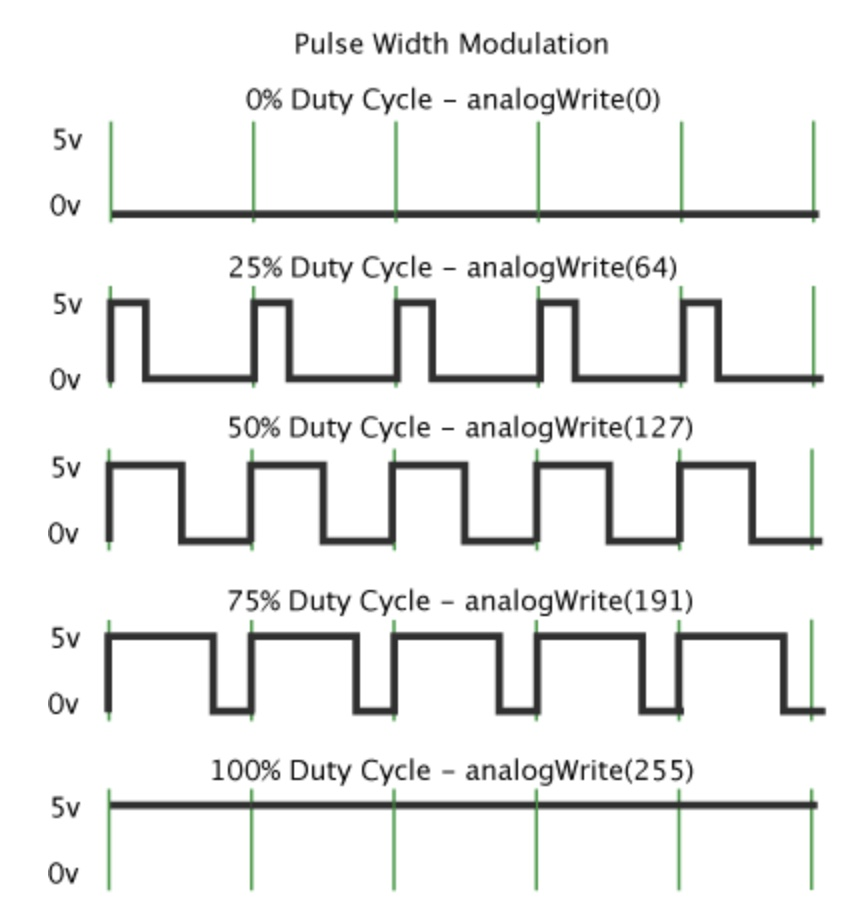
\includegraphics [width=13cm, height=8cm] {img/pulsweite} \newline \newline
Spezifischer ausgedrück passiert folgendes:
Eine Digitale Steuerung wird verwendet, um eine Rechteckwelle - ein Signal das zwischen Ein und Aus umgeschaltet wird
- zu erzeugen. Dieses Ein-Aus-Muster kann Spannungen zwischen der vollen Versorgungsspannung und Aus
simulieren.
Dabei wird der Anteil der Zeit geändert, den das Signal eingeschaltet ist im Vergleich zur Zeit, die das Signal
ausgeschaltet ist. Die Dauer der Einschaltzeit wird als Pulsweite bezeichnet. Um unterschiedliche analoge Werte zu
erhalten, wird die Pulsweite geändert bzw. moduliert. Wenn dieses Ein-Aus-Muster zum Beispiel schnell genug mit einer LED
wiederholt wird, resultiert daraus eine konstante Spannung zwischen 0 und Vcc, die die Helligkeit
der LED steuert. \newline
Auf den Arduino bezogen sieht die Umsetzung eines PWM Signals wie folgt aus:
Ein Taktsignal gelangt in die entsprechende Clock.
Die Clock stellt den entsprechenden PWM-Modus ein. Dabei werden zwei wichtige Werte gesetzt:
Der erste bestimmt, wann das Signal von HIGH auf LOW
umschaltet, während der zweite bestimmt, wann es zurückkommt. Das Verhältnis zwischen HIGH und LOW wird als
Tastverhältnis bezeichnet und bestimmt die Helligkeit unserer LED bzw. die Stärke, mit welcher der Hubmagnet anschlägt.
Je länger die Ausgabe im HIGH-Zustand bleibt, desto schneller erfolgt der Tastenanschlag. \newline
Neben dem Tastverhältnis, also das Verhältnis der Einschaltzeit zur
Periodendauer, welches oft in Prozent ausgedrückt wird, ist auch die Resolution (de: Auflösung) ein variierbarer Parameter.
Die Resolution bezieht sich auf die Anzahl der möglichen diskreten Werte, die das Signal annehmen kann.


\subsection{Vermehrung der Ausgänge}\label{output}
Da ein Klavier über 88 Tasten verfügt, müssen 88 Aktuatoren angesteuert werden. Ein Arduino hat keine 88 PWM-Ports, daher
müssen die Signale über eine Erweiterung der Ausgänge an die Motoren weitergegeben werden. Dafür gibt es mehrere Möglichkeiten:

\begin{enumerate}
	\item Schieberegister
	\item Motor-Matrix
	\item Demultiplexer
\end{enumerate}

\paragraph{Schieberegister}
Ein Schieberegister ist ein integrierter Schaltkreis, der hier verwendet wird, um die Anzahl der verfügbaren Ausgänge des
Mikrocontrollers zu erweitern. \newline
Um 88 Ausgänge mit Hilfe von Schieberegistern von nur 3 PWM-Pins des Arduinos anzusteuern, werden insgesamt 11 8-Bit-Schieberegister
(Also Schieberegister mit 8 Ausgängen) benötigt.\newline

Zuerst werden die Datenleitungen (SERIAL IN) aller Schieberegister in Reihe geschaltet. Dies bedeutet, dass das
Ausgangssignal des ersten Schieberegisters mit dem Eingang (SERIAL IN) des nächsten verbunden wird, und so weiter, bis
zum letzten Schieberegister. \newline
Der Arduino sendet Daten seriell über die verbundenen PWM-Pin. Diese Daten werden über ein Schieberegister an
alle Schieberegister weitergegeben. Durch diesen Vorgang werden die Daten parallel über alle Schieberegister gesendet.
\newline
Die Ausgänge der Schieberegister (Q0 bis Q7) werden dann an die entsprechenden Aktuatoren angeschlossen.
Das Signal wird zu einer definierten Clock durch die Schieberegister durchgeschoben. So kann durch Steuerung der Daten,
die an die Schieberegister gesendet werden, kann der Arduino jeden einzelnen Ausgang manipulieren, um die Aktuatoren
entsprechend anzusteuern. \newline
Auf diese Weise kann der Arduino mit Hilfe von Schieberegistern eine größere Anzahl von Ausgängen kontrollieren, als er
direkt verfügbar hat.


\paragraph{Motor-Matrix}
Die Motor-Matrix ist einer LED-Matrix nachgeahmt. //TODO: Picture Matrix and use muster to explain it for magnets
In einer Matrix, werden zwei Reihen an Ports angeschlossen, nach folgendem Muster:
$$
\begin{pmatrix}
	(11) & (12) & (13) & (14) & (15) & (16) & (17) & (18) \\
	(21) & (22) & (23) & (24) & (25) & (26) & (27) & (28) \\
	(31) & (32) & (33) & (34) & (35) & (36) & (37) & (38) \\
	(41) & (42) & (43) & (44) & (45) & (46) & (47) & (48) \\
	(51) & (52) & (53) & (54) & (55) & (56) & (57) & (58) \\
	(61) & (62) & (63) & (64) & (65) & (66) & (67) & (68) \\
	(71) & (72) & (73) & (74) & (75) & (76) & (77) & (78) \\
	(81) & (82) & (83) & (84) & (85) & (86) & (87) & (88)
\end{pmatrix}
$$


Eine LED-Matrix besteht aus einer Anordnung von LEDs in Zeilen und Spalten. Jede LED kann unabhängig von den anderen
ein- oder ausgeschaltet werden. Die Steuerung erfolgt über Multiplexing, bei dem jede Zeile der Matrix nacheinander
aktiviert wird, während die entsprechenden LEDs in den Spalten gleichzeitig eingeschaltet werden. Durch schnelles
Wechseln zwischen den Zeilen (PWM) erscheint es den BetrachterInnen, als ob alle LEDs gleichzeitig leuchten würden,
obwohl sie tatsächlich nacheinander aktiviert werden. \newline

Um das Prinzip einer LED-Matrix auf Aktuatoren zu übertragen, müssen lediglich die LEDs durch die Aktuatoren ersetzt werden.
Durch Steuerung der Zeilen und Spalten dieses Rasters können verschiedene Motoren selektiv
aktiviert werden. Dies ermöglicht eine effiziente Steuerung mehrerer Motoren mit einem begrenzten Satz von
Steuersignalen. \newline

//TODO: Nachteile Matrix


\paragraph{Demultiplexer}
//TODO

\subsection{Transistor}
Durchlaufspannung, Mindestspannung
\subsection{Aktuator}\label{subsec:aktuator}

\subsection{Schaltplan}

\textit{Arduino}

Im Zentrum der Schaltung steht der Mikrocontroller (hier: Arduino Uno R3).
Dieser erhält Daten und Strom über den integrierten USB-Anschluss, welcher mit dem Computer verbunden wird.
Da der Arduino limitierte \nameref{PWM}-fähige Ausgänge bereitstellt, werde Schieberegister (74HC595) verwendet.
Mit jedem \"in Reihe" geschaltetem Schieberegister kann die Anzahl PWM-fähiger Ausgänge um 8 erweitert werden.

\textit{Schieberegister}

Der Arduino wird an fünf Stellen mit dem ersten Schieberegister verbunden:

Arduinoport D2 <-> Serial (SER) Input

Über diese Verbindung werden serielle Daten werden hier bitweise in das Register geschoben.

Arduinoport D3 <-> SHCP (Shift Register Clock Input)

Dieser Pin wird verwendet, um den Takt für das Verschieben der Daten innerhalb des Schieberegisters anzulegen.
Bei jedem Taktimpuls auf diesem Pin wird das Bit am seriellen Dateneingang in das Register verschoben.
Das bedeutet, dass bei jeder steigenden Flanke des Taktsignals das Datenbit, das am Eingang anliegt, in das Schieberegister übernommen und alle vorhandenen Daten um eine Position verschoben werden.

Arduinoport D4 <-> STCP (Storage Register Clock Input)

Nachdem die Daten in das Schieberegister eingelesen wurden, wird dieser Pin verwendet, um die im Schieberegister vorhandenen Daten in das Ausgangsregister zu übertragen.
Ein Taktimpuls auf diesem Pin bewirkt, dass die Daten vom Schieberegister ins Ausgangsregister übernommen werden, sodass alle Ausgänge gleichzeitig aktualisiert werden.
Das ist besonders relevant, da sonst unter Umständen alle Ausgänge von einer Änderung im letzten Schieberegister bedingst wären.

Arduino GND <-> Ground, Output Enable (OE)

Der OE-Pin wird genutzt, um die Ausgänge des Schieberegisters global zu aktivieren oder zu deaktivieren, ohne die Daten selbst zu beeinflussen.
Da das Schieberegister zu keiner Zeit deaktiviert sein soll, wird dieser Pin dauerhaft mit dem GND-Pin verbunden.

Arduino VCC 5V <-> VCC, $\overline{SRCLR}$ (Reset)

Um das Schiebregister mit den benötigten 5V zu betreiben, wird der entsprechende Pin mit dem 5V Output des Arduino verbunden.
Zusätzlich wird der $\overline{ }$ SRCLR Port des Schieberegisters, welcher ein Reset ermöglicht dauerhaft mit 5V verbunden.

Jedes weiteres Schieberegister greift die oben genannten Signale ab.
Der einzige Unterschied befindet sich am Serial (SER) Input Port.
Das Schieberegister an Position i+1 wird mit dem seriellen Output des Schieberegisters an Position i verbunden. ($\forall i = 0,...,10$)

\textit{MOSFET}

Die Hubmagnete werden jeweils mit 24V und mit bis zu 400mA betrieben.
Um einen hohen Stromfluss zu steuern, können Transistoren verwendet werden.
Für hohe Spannungen und schnelle Schaltvorgänge eigenen sich besonders MOSFETs (Metall-Oxid-Halbleiter-Feldeffekttransistor).
Im Folgenden werden speziell n-MOSFETs verwendet, der mit einem Signal zwischen 0V (leitet nicht) und +5V (voll leitend) angesteuert werden kann.

Der folgende Aufbau ist für die insgesamt 88 Ausgänge der 11 Schieberegister identisch, da jeder Ausgang für die Ansteuerung genau eines Motors zuständig ist.

Der GATE-Pin des MOSFETs erhält das Signal, dass die \"Durchlässigkeit" steuert aus einem der Outputs des Schieberegisters.
Der SOURCE-Pin wird mit Ground des gesamten Systems verbunden.
Der DRAIN-Pin wird direkt mit dem entsprechenden Kontakt am Hubmagneten verbunden.

\textit{Hubmagnet}

Um den Stromkreis zu schließen wird der andere Kontakt des Hubmagnetes mit dem +24V verbunden.

\textit{Testen}

Um die Fehlersuche zu erleichtern, werden LEDs in den Schaltplan mit eingebaut.
Diese werden jeweils mit einem entsprechenden $1k\Omega$ Widerstand parallel zu den Motoren angeschlossen.
So kann anhand der Helligkeit der LED die Intensität abgelesen werden, mit der eine Taste gespielt wird.

//Bild vom Schaltplan

\section{Mechanik}\label{vorgehenHW}

\subsection{Auswahl des Klaviers}

Da sich dieses Projekt nicht auf die theoretische Konzeption beschränkt, muss ein entsprechendes Testobjekt - ein reales Klavier - gefunden werden.
Dieses muss einige Voraussetzungen erfüllen:
\begin{enumerate}
	\item 	Der Preis muss im Rahmen des Budgets (gesamt < 2000 €) liegen
	\item 	Es muss leicht auseinander zu bauen sein, um die Mechanik zugänglich zu machen
	\item 	Es muss vollständig sein (alle 88 Tasten)
	\item 	Es muss stimmbar sein
	\item 	Der Transport muss einfach durchzuführen sein
\end{enumerate}


\subsection{Ansteuerungskonzept}

//Drücken der ziehen, oben oder unten...
1. Oben
	Klavierhand
	Schiene
	Aufsatz mit 88 oben drüber
2. unten
	ziehen
	drücken

\subsection{Anbringung der Aktuatoren}
Beim Ansteuerungskonzept der Tasten muss auch beachtet werden, wo die Magnete befestigt werden.
Wir haben ein Brett, auf welchem sie befestigt werden. Folgende Bedenken:
1. Wie viel Platzt zwischen Solenoids?-weil Hitze
bsp. weiß unten und schwarz oben, weil die weißen weiter vorne
	-> nicht weil funktionalität vor optik (weil zu eng)
 -> Platz maximieren

2. Wie verbinden ohne dass Angelschnuren und andere Solenoids sich in den weg kommen
(3. spezifischer . in 2 oder 3 Reihen)
Voteil: Hitze
Nachteil: Umlenkung, Verkabelung

4. Umlenkung, damit der ganze Hub verwendet werden kann

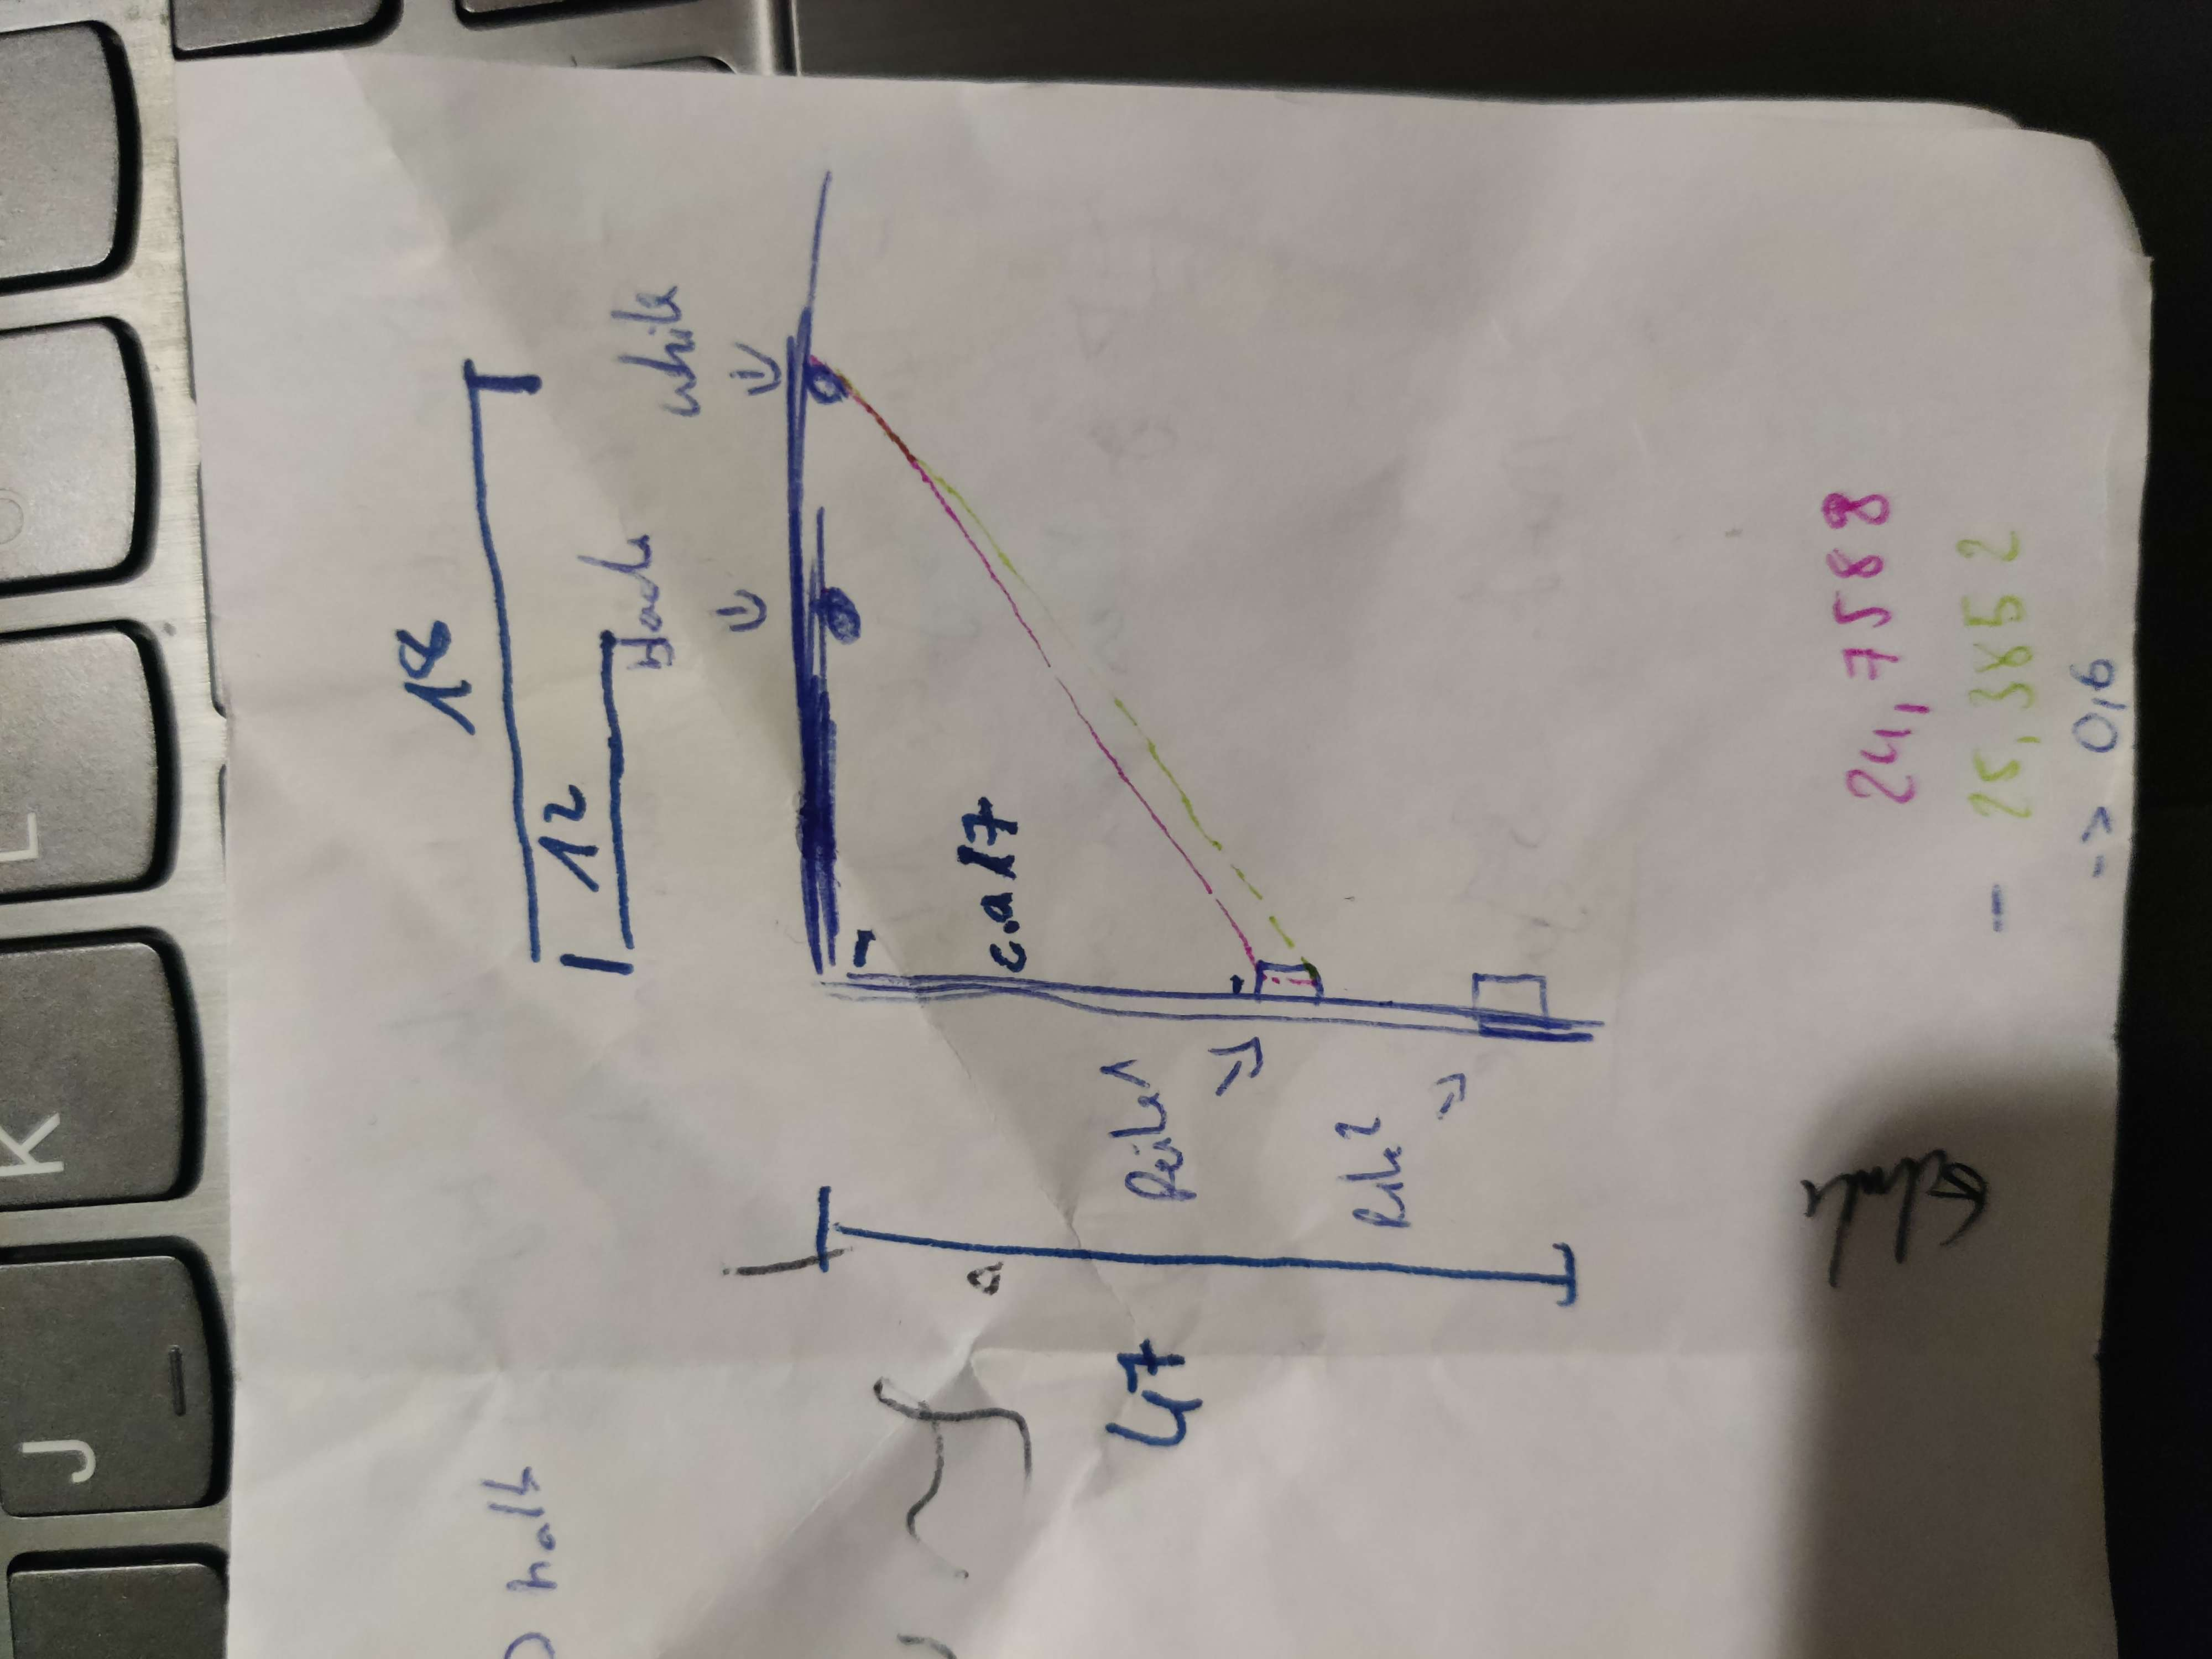
\includegraphics [width=5cm, height=4cm,angle=-90] {img/skizze_Umlenkung}

*Bild wegen Umlenkung

Erklärung geben: Haben Brett mit 67x25cm für 44 Motoren
*Bild von Brett-Sikzze



\subsection{Verbindung Tasten und Hubmagnete}

Es wurde sich dazu entschieden die Tasten durch Ziehen anzusprechen (siehe:\nameref{Ansteuerung}).
Die Grundidee ist, eine Schnur, oder Ähnliches, durch ein waagerechtes Loch in der Taste zu befestigen.
Anschließend wird die Schnur durch ein senkrechtes Loch durch das Holz, worauf die Tasten liegen, in den Fußraum geführt.
Damit der Pianist:in nicht durch Platzmangel eingeschränkt wird, werden die Seile entlang der Verkleidung zum Rumpf des Klaviers geführt.
Dort werden die Hubmagnete über die gesamte Breite befestigt.
Um die Intensität des Tastendrucks zu steuern und die Durabilität des Materials zu verlängern, sollte die Reibung möglichst gering gehalten werden.
Dazu wird mittels eines Rohres, welchen waagerecht unter der Klaviatur entlang der Löcher montiert wird als erste Umlenkung verwendet.


Für das Ziehen wird ein leichtes, formbares und dünnes Material benötigt, da Konzept die eine Seite mit dem Motor und die andere durch ein Loch in der Taste verknotet werden sollte.

\textit{Nähgarn}

Als Erstes wurden Nähgarn, welches zur Hand war getestet.
Auch doppelt hielt es der ruckartigen Ziehbewegung mit 25N des Hubmagnetens nicht stand.
Vier Fäden funktionierten zu Beginn gut, leierten allerding schnell aus.

\textit{Nylonsaiten}

Als Nächstes wurde die g-Saite einer Gitarre verwendet.
Durch den höheren Durchmesser und das stärkere Material riss und leierte die Saite nicht aus.
Da die Saite kaum Flexibilität liefert, war die Befestigung an der Taste äußerst schwierig.
Dadurch konnte nicht der vollständige Hub des Magnetes auf die Taste übertragen werden.

\textit{Angelschnur}

Aus Erfahrungen aus dem Angelbereich konnte schnell eine geeignete Schnur gefunden werden.
Genauer handelt es sich um eine geflochtene Schnur aus Polyethylene.
Mit einem Durchmesser von 1.6mm ist sie nicht nur sehr dünn und flexibel, sondern kann auch bis zu 7kg standhalten.
Damit sollte das Spielen des Forellenquintetts von Schubert ein leichtes sein.



\subsection{Weitere Ideen und Limitationen}

Im Laufe der Konzeption traten mehrere Herausforderungen auf, welche aus Zeit- und Konsten- Gründen nicht weiter
behandelt wurden.
\paragraph{Anzahl der Aktuatoren}
Wie bereits erklärt, wurden insgesamt 88 Aktuatoren verbaut, womit jede Taste angespielt werden kann. Trotz der Anzahl an
Hubmagneten, werden maximal 10 Tasten glechzeitig angespielt. Dies liegt an der Stromversorgung. Ein Hubmagnet benötigt
eine Stromversorgung von etwa 0.4 Ampere, für 10 Aktuatoren sind das also 4 Ampere. Das Netzteil welches wir verwenden, ist auf
6(?) Ampere ausgelegt, wobei wir mit einem Netzteil getestet haben, welches 2,8 Ampere unterstützt. Es gibt Netzteile die
einen höheren Stromföuss ermöglichen, allerdings sind diese um weiten teurer als das Netzteil, für welches wir uns entschieden haben.
Es wäre auch möglich, ein zweites Netzteil parallel zu Schalten, wodurch die Kosten nicht dramatisch gestiegen wären.
Wir haben hier allerdings keinen Mehrwert mehr gesehen. Die Logik und Ansteuerung des Klaviers bleibt die gleiche, weswegen
wir bei einem Netzteil mit einem maximalen Stromfluss von 6 Ampere (und 24V Leistung) verblieben sind.

\paragraph{Pedalansteuerung}
Ein Klavier hat normalerweise zwei oder drei Pedale, welchedie dynamik und den Klang des Klaviers beeinflussen.
Diese sind schwerer anzuspielen als die Tasten und benötigen somit Leistungsfähigere Aktuatoren als wir für die
Tasten nutzen. Es gab eine Überlegung diese Aktuatoren zu besorgen, da die Pedale klangtechnisch Mehrwert bringen.
Außerdem hätten wir uns noch Gedanken bezüglich der Schaltug und des Signals machen können. Einerseits hätte ein weiteres
Schieberegister genutzt werden können, wobei das Signal angepasst wird das die letzten 6 Ausgänge nie ein Signal bekommen.
ANdererseits hätten die Pedale mit weiteren PWM Ports des Arduinos verbunden werden können und die Signale unabhängig von den
Schieberegistern erhalten können. Im Prinzip wäre die Idee hier allerdings wieder die selbe wie beim Rest des Projektes gewesen,
weswegen wir Kosten an den Aktuatoren und der extra Stromversorgung für die Pedale gespart haben und diese nicht ansteuern.

\paragraph{Klangdämpfung der Aktuatoren}
Die Hubmagnete machen beim Anschlagen Geräusche, welche von der Melodie des Klaviers ablenken. Es gab eine Überlegung,
diese zu Dämpfen undem das Innere der Hubmagnete mit Isolierfolie abgedeckt wird und die Geräusche somit nicht so
offensichtlich sind. Letztendlich war uns die Gefahr, dass die Hubmagnete durch die Isolierung überhitzen oder nicht ganz
zurück schellen zu hoch, als dass wir die Klangdämpfung umsetzen würden.

Notiz von Oli: siehe diy piano Anschlag dempfen, indem man mit gummi die Taste limitiert
Notiz von Oli: Motorlager verwenden zwischen Platte und Klavier
Notiz von Oli:
Aktuatoren Geräuschreduzierung Tests:

Weg normal: 10mm

1. Schaumstoff:

*siehe bild
reduzierung des Weges, abfangen bevor es klopft
hässlich
sehr leise
Weg: 9mm (-1)

2. Seil (2mm Durchmesser) um den Anker

kann nicht rutschen, da kante
Nachteil: reibung
sehr leise
Weg: 8mm (-2)
%%%%%%%%%%%%%%%%%%%%%%%%%%%%%%%%%%%%%%%%%%%%%%%%%%%%%%%%%%
%   Autoren des Abschnitts:
%   Jakob Kautz
%   Olivier Stenzel
%%%%%%%%%%%%%%%%%%%%%%%%%%%%%%%%%%%%%%%%%%%%%%%%%%%%%%%%%%

% !TEX root =  master.tex
\chapter{Umsetzung - Hardware} \label{umsetzungHW}
\chapterauthor{Jakob Kautz, Olivier Stenzel}

\nocite{*}
- Probleme, Schwierigkeiten, Änderungen während der Umsetzung

Nachdem die Planungsphase abgeschlossen war, mussten die Überlegungen umgesetzt werden.
Im Rahmen dieser Arbeit wurde ein Prototyp gebaut, welcher 8 Tasten anspielen kann.
Zusätzlich wurde die Elektronik mit LEDs so erweitert, dass man das Drücken von 40 Tasten simulieren kann. % @Note(Val): Entweder hier oder an späterer Stelle erwähnen, dass es an sich trivial aber halt zeitaufwendig wäre, mehr Tasten anspielbar zu machen
% @Note(Val): Ich würde hier vielleicht noch gar nicht erwähnen, dass nur 8 Tasten anspielbar sind, weil die ganze Umsetzung ja mit dem Ziel 88 Tasten anspielbar zu machen lief. Kostenschätzung, etc. sind deshalb ja auch höher. Vielleicht ist es besser hier zu sagen, dass das Ziel war, den Prototypen mit möglichst vielen spielbaren Tasten zu gestalten, aber nur 8 bis dato erledigt wurden

\section{Materialien}
\chapterauthor{Jakob Kautz}
\subsection{Liste der Bauteile}
%TODO(Jay): Fix List
\begin{table}[htbp]
    \centering
    \begin{tabular}{|m{3.8cm}|m{1.7cm}|m{8cm}|}
        \hline
        \textbf{Bauteil} &  \textbf{Anzahl} & \textbf{Begründung}  \\
        \hline
        Hubmagnete & 88 & jede Taste braucht einen Hubmagneten um angespielt zu werden \\ % @Note(Val): Erwähnen, dass nur 8 der Hubmagnete benötigt wurden
        \hline
        Stromversorgung & 1 & Externe Stromversorgung für die Aktuatoren, da diese mehr als die 5V Vcc des Arduinos brauchen \\
        \hline
        Arduino & 1 & Kommunikation \\
        \hline
        Breadboard & 2 & Kleinstromschaltung \\
        \hline
        Schaltplatine & 5 & Großstromschaltung\\ % @Note(Jay): Heißt das so?
        \hline
        Schieberegister & 11 & Weitergabe Signal\\
        \hline
        Kabel (10cm) & 352stck (bzw. $9\cdot40$ in Packs) & Verbindungen in der Schaltung mit Schätzung 4 Kabel pro Hubmagnet\\
        \hline
        Kabel (20cm) & 176stck (bzw.$5\cdot40$ in Packs) & Verbindungen zu den Hubmagneten \\
        \hline
        LEDs & 88 & Tests \\
        \hline
        1kOhm Widerstände & 90 & Sicherheit and shit \\
        \hline
        MOSFET & 90 & Steuerung Strom \\
        \hline
        Feste Anschlussblöcke & 88 & Anschluss von Schaltplatine zu Hubmagnet\\
        \hline
        Angelschnur (...cm) & 88 & Verbindung Hubmagnet und Taste \\
        \hline
    \end{tabular}
    \caption{Ergebnisse der Anforderungen}
    \label{table:Bauteile}
\end{table}

\subsection{Kostenübernahme}
Die vorher spezifizierte Hardware für den Schaltplan musste für die Erstellung des Prototypen offensichtlich besorgt werden.
Aufgrund der relativ hohen Kosten für eine Studienarbeit, wurde bei einer der betreuenden Firmen angefragt, ob diese die Kosten für das Projekt übernehmen würde.
Damit dies möglich war, wurde ein Kostenvoranschlag gestellt, in welchem die benötigten Materialien mit den geschätzten Kosten aufgeführt wurden. % @TODO(Val): Kostenanschlag wird wahrscheinlich eine Tabelle, also referenzier die einfach "(siehe Tabelle \ref{...})" oder so

% @TODO(Jay): Add Kostenschätzung

Der Kostenanschlag erwies sich im Laufe des Projektes als (teils) unrealistisch. Dies lag insbesondere an der Anforderung
der Firma. Die Schätzung der Kosten basierte auf Anbietern, bei welchen die Materialien möglichst günstig zu kaufen sind.
Durch Firmenreglungen mussten diese allerdings alle bei Conrad oder Reichelt
% @Note(Jay): Stimmt das so?
gekauft werden. Diese Anbieter verkaufen die Materialien für sehr viel mehr Geld. Die tatsächlichen Kosten liefen
letztendlich also auf folgende Beträge hinaus: \newline % @TODO(Val): Hier am besten auch einfach wieder nur die Tabelle referenzieren, statt sie unbedingt in die nächste Zeile zu quetschen
% @TODO(Jay): Tatsächliche Kosten

Der Kostenunterschied betrug daher insgesamt .
% @TODO(Jay): Add difference
Hierbei ist allerdings zu erwähnen, dass die Kostenschätzung passend gewesen wäre, wenn die Anbieter frei wählbar wären.

\section{Prototypenbau}
Ursprünglich sollte der Aufbau des in Kapitel \ref{subsec:schaltplan} spezifizierten Schaltplans via Steckbrettern und
Jumperkabeln umgesetzt werden.
Zu Beginn wurde dies auch so umgesetzt. Das Problem welches dadurch entstand, war, dass die gewählten Platinen den
benötigten Stromfluss nicht aushalten.\newline
Jeder Aktuator - also jede gedrückte Taste - zieht einen Strom von 0.7A. Um das Projekt möglichst sinnvoll umzusetzen,
sollte der Aufbau mindestens 10 Tasten gleichzeitig drücken können, was bedeutet, dass der Aufbau mindestens 7.0A
Stromfluss problemlos ausstehen muss.
% @TODO(Jay): Wie viel halten Platinen aus? Warum konnten wir ein paar Jumper-Kabel nutzen? Wann brauchten wir die dickeren? Tabelle für welche Kabeldicke für welchen Stromfluss
% @Note(Val): Wann haben wir entschieden, dass min. 10 Tasten gleichzeitig spielbar sein sollen? Wenn wir das als Anforderung haben wollen, muss das im Anforderungs-Kapitel auch erwähnt werden

Aus diesem Grund wurde die gesamte Schaltung, die nach dem Schieberegister kommt, auf einer Lochrasterplatine fest gelötet.
Hierfür wurde ein 3mm starker Draht für die Stromversorgung verwendet.

\subsection{Klavieranbau}
Im Rahmen des Protoypen wurde die Elektrik nicht fest am Klavier verschraubt.
Das Brett mit den Hubmagneten wurde stattdessen nur an das Klavier angelehnt, während die Angelschnüre die Verbindung zu den Tasten herstellen.
Gespannt werden die Seile durch eine Schrauben-Mutter Konstruktion (siehe Abschnitt \ref{subsec:VerbindungTastenAktuatoren}).

\subsection{Ergebnisse des Prototypen}
% @TODO(Val):
Das Anspielen klappt iwie aber noch hakelig.


  \acresetall % Reset acronym definitions between hardware-software transition section
%%%%%%%%%%%%%%%%%%%%%%%%%%%%%%%%%%%%%%%%%%%%%%%%%%%%%%%%%%
%   Autoren des Abschnitts:
%   Val Richter
%%%%%%%%%%%%%%%%%%%%%%%%%%%%%%%%%%%%%%%%%%%%%%%%%%%%%%%%%%

% !TEX root =  master.tex
\chapter{Konzeption - Software} \label{vorgehenSW}
\chapterauthor{Val Richter}

Wie in Kapitel \ref{Zielstellung} beschrieben, soll eine Desktop-Anwendung für die Nutzer-Interaktion mit dem \enquote{Piano Player} erstellt werden.
Die Anwendung soll im Folgenden auch als \enquote{\acf{SAM}} bezeichnet werden.
Die fundamentale Aufgabe der Anwendung liegt im Verwalten und Spielen von Musikstücken auf dem selbstspielenden Klavier.
Zum Anspielen des Klaviers wird ein \acf{MC} benötigt (siehe Kapitel \ref{Ansteuerung}).
Da die Auswahl des Musikstücks dynamisch während der Laufzeit über \acf{SAM} gehen soll, muss \ac{SAM} mit dem \ac{MC} kommunizieren können.
In diesem Kapitel soll die Software beider Komponenten und deren Kommunikation konzipiert werden.

Abbildung \ref*{fig:high-level-komponenten} zeigt diese unterschiedlichen Komponenten, sowie den Datenfluss zwischen diesen.
Nutzer:innen werden in der Abbildung auch dargestellt, um eindeutig zu machen, dass Nutzer-Eingaben nur an \ac{SAM} gehen.
Der \ac{MC} erhält Daten zum abzuspielenden Musikstück von \ac{SAM} und schickt darauf basierend in regelmäßigen Intervallen \ac{PWM}-Signale an den \enquote{Piano Player}.

\begin{figure}[htbp]
    \centering
    \begin{tikzpicture}[node distance=2cm, line width=0.25mm]
        \node (user) [rect] {User};
        \node (ui) [rect, below of=user] {\ac{SAM}};
        \node (mc) [rect, right of=ui, xshift=1.5cm] {\ac{MC}};
        \node (hw) [rect, right of=mc, xshift=1.5cm] {Piano Player};

        \draw [arrow] (user) -- (ui);
        \draw [arrow] (ui)   -- (mc);
        \draw [arrow] (mc)   -- (hw);
    \end{tikzpicture}
    \caption{Komponenten-Diagramm mit Datenfluss}
    \label{fig:high-level-komponenten}
\end{figure}

Da die Hardware-Komponente in vorherigen Kapiteln bereits behandelt wurde, soll hier nur die Architektur der Desktop-Anwendung (in Abschnitt \ref{vorgehenSW-UI}) und des \ac{MC}s (in Abschnitt \ref{vorgehenSW-MC}) erarbeitet werden.
Weiterhin soll noch die Kommunikation zwischen diesen beiden Komponenten in Abschnitt \ref{vorgehenSW-SPPP} betrachtet und spezifiziert werden.
Ein Ziel der Kommunikations-Spezifikation ist eine leichte Anpassbarkeit der einzelnen Komponenten, solange sie sich weiterhin an das selbe Kommunikations-Protokoll halten.
Damit soll der Anforderung A8 gerecht werden.

Da die Konzeption aller Teile jedoch vom Format, in dem Musikstücke auf dem \ac{MC} gespeichert werden, abhängen, soll dieses zuerst entworfen werden (siehe Abschnitt \ref{vorgehenSW-PIDI}).
Da der \ac{MC} eine möglichst hohe Geschwindigkeit für die Ansteuerung der Motoren erbringen soll, muss das Format eine performante Nutzung ermöglichen.
Auch muss das Format möglichst wenig Speicherplatz aufbrauchen, damit möglichst viele Daten auf einmal auf dem \ac{MC} gespeichert werden können.
Je mehr Speicherplatz das Format nämlich benötigt, desto öfter muss die \ac{UI} Daten an den \ac{MC} schicken, was aufgrund relativ hoher Latenzen in der Kommunikation nicht wünschenswert ist.


\section{Datenformat für Musikstücke} \label{vorgehenSW-PIDI}

Es gibt bereits viele Datenformate, die zum Speichern von Musikstücken verwendet werden können. Dabei lassen sich solche Formate generell in zwei fundamental verschiedenen Designs unterscheiden.

Zum Einen gibt es generelle Audioformate. Dazu gehören solche Formate wie MP3\footnote{formal \enquote{MPEG-1 Audio Layer III} bzw. \enquote{MPEG-2 Audio Layer III}; siehe \cite{iso.MP3} für die Spezifikation des Formats}, WAV\footnote{wird auch \enquote{WAVE}-Format genannt; siehe \cite{kab.WaveFileSpecifications.22} für die Spezifikation des Formats} oder FLAC\footnote{formal \enquote{Free Lossless Audio Codec}; siehe \cite{bw.FLAC.24} für die Spezifikation des Formats}.
Diese Formate speichern für jeden Zeitpunkt des Audios die Information über das Geräusch, das zu diesem Zeitpunkt abzuspielen ist.

Zum Anderen gibt es Formate, die speziell für Musikstücke entwickelt wurden.
Das Vorzeige-Beispiel wäre hier das \ac{MIDI}-Format.
Bei diesen Formaten werden statt Geräusch-Daten Informationen über Noten, die für eine gewisse Zeit zu spielen sind, gespeichert.
Das genaue Geräusch, das am Ende abgespielt werden sollte, wird dabei noch von anderen Faktoren beeinflusst.
So könnten beispielsweise mehrere Noten gleichzeitig zu spielen sein.
Auch könnte das Instrument von Nutzer:innen dynamisch änderbar sein.

Die zweite Art an Formaten ist im Kontext dieses Projekts zu bevorzugen, da es dem Format der Ausgabe näher kommt.
Zum Anspielen eines Klaviers werden nämlich zu jedem Zeitpunkt die Information über derzeit zu spielende Tasten benötigt.
Formate der zweiten Art speichern genau jene Informationen und erfordern damit keine weiteren Informations-Umwandlungen mehr. \newline
Im Gegensatz dazu sind die erstgenannten Formate speziell für digitale Lautsprecher entworfen worden und speichern entsprechend Informationen über die vom Lautsprecher zu spielenden Geräusche.

Wenn hier von Informations-Umwandlung gesprochen wird, meint dies nicht eine simple Datentransformation.
Daten sind eine Enkodierung von Informationen und somit können unterschiedliche Daten die selben Informationen darstellen.
Die Wandlung eines Datensatzes in eine andere Kodierung kan zwar rechenaufwendig werden, ist aber ohne Verlust von Informationen möglich.
Je nach Kontext können Datentransformationen auch ausgelassen oder stark optimiert werden.
Falls grundlegend andere Informationen benötigt werden, ist eine Änderung der Daten nicht nur notwendig, sondern oftmals auch vergleichsweise aufwendig.

Es ist also festzuhalten, dass die Verwendung eines Formats wie \ac{MIDI} hier sinnvoll ist.
Bevor \ac{MIDI} selbst gewählt wird, sollten jedoch noch weitere Aspekte beachtet werden.

Eine Anforderung dieses Projekts ist eine höhere Performanz als die schnellsten menschlichen Pianist:innen zu erreichen (siehe Tabelle \ref{table:anforderungen}).
Entsprechend sollte das gewählte Datenformat der Musikstücke auch möglichst schnell in das Format umgeformt werden können, das für die Ausgabe an die Aktuatoren benötigt wird.
Am performantesten wäre es hierbei, eine Liste jener Daten zu speichern, die zu jedem Zeitpunkt an die Aktuatoren ausgegeben werden müssen, da dann gar keine Datentransformation mehr nötig ist.

Allerdings muss das Datenformat auch möglichst wenig Speicherplatz verbrauchen.
Da der Code auf einem \ac{MC} laufen muss, ist Speicherplatz relativ begrenzt.
Der \ac{MC} muss dabei nicht das gesamte Musikstück auf einmal gespeichert haben, da restliche Teile des Musikstücks auch später von \ac{SAM} nachgereicht werden können.
Das verringert die Wichtigkeit des Speicherplatzes jedoch nur zu Teilen, da ein solches Streamen der Daten mehr Kommunikation zwischen \ac{SAM} und {MC} benötigt.
Da die Latenzen der Kommunikation relativ hoch sein können, gefährdet dies wiederrum das Ziel der Performanz\footnote{Während der Erstellung der Konzeption wurde experimentell herausgefunden, dass die Latenzen nicht zu vernachlässigen sind. Konkrete Zahlen wurden jedoch erst bei den Tests am Ende der Entwicklung ermittelt und finden sich in Tabelle \ref{table:sw-tests}}.

\ac{MIDI} schneidet hierbei an sich sehr gut ab, da Noten sehr kompakt abgespeichert werden.
Dafür wird eine Enkodierung variabler Länge verwendet \cite[vgl.][S. 131]{mid.CompleteMIDIDetailed.96}.
Da \ac{MIDI} allerdings ein generelles Format ist, das eine Vielzahl von digitalen Instrumenten und Synthesizers unterstützen möchte, beinhaltet der \ac{MIDI}-Standard eine Vielzahl optionaler Metadaten \cite[siehe][für die gesamte Liste]{vm.ControlChangeMessages.20}, die für dieses Projekt irrelevant sind.
Entsprechend würde nur ein Subset des \ac{MIDI}-Standards zum Speichern der Musikdaten in Frage kommen. \newline
Nichtsdestotrotz kann das Format für diesen eingeschränkten Anwendungsfall noch optimiert werden.
Um diese Verbesserungen zu motivieren, soll zuerst die Enkodierung von Noten in \ac{MIDI} erläutert werden.

\ac{MIDI} speichert die Notenfolgen in sogenannten \enquote{Nachrichten}.
Nachrichten können auch andere Daten tragen \cite[siehe][für die gesamte Liste]{vm.SummaryMIDIMessages.20}, hier sollen aber nur die Nachrichten zum Spielen von Tönen betrachtet werden.
Jede dieser Nachrichten folgt einer relativen Zeitangabe, im Standard \enquote{delta time} genannt.
\enquote{delta time} gibt an, wie viele Schläge der virtuellen \ac{MIDI}-Uhr zwischen der letzten Nachricht und dieser vergehen sollen.
Die \ac{MIDI}-Uhr kann direkt in Angaben einer Wand-Uhr umgerechnet werden.
Hier ist jedoch wichtig zu bemerken, dass diese \ac{MIDI}-Uhr sehr viel genauer als eine Angabe in Millisekunden ist.
Auch ist zu erwähnen, dass diese \enquote{delta time} eine variable Länge hat, mindestens aber immer ein Byte verwendet \cite[vgl.][S. 135]{mid.CompleteMIDIDetailed.96}.

Nach der \enquote{delta time} folgt dann genau ein Byte für den \enquote{Ereignis-Code} der Nachricht.
Dieser gibt in jeweils 4 Bits den \enquote{Status} und den \enquote{Kanal} des Ereignisses an.
Während der Status angibt, was für eine Aktion ausgeführt werden soll und damit auch wie viele Datenbytes für diese Nachricht noch folgen, besagt der Kanal, für welches Instrument dieses Ereignis gilt.
Beim Anspielen und Aufhören des Spielens einer Note folgen jeweils zwei Bytes, die respektiv die Note und Spielstärke angeben \cite[vgl.][Kapitel 2]{van.MIDITutorialProgrammers.12}.

Hierbei fallen einige Daten auf, die in diesem Projekt unnötig sind.
So gibt es hier zum Beispiel nur ein einziges Instrument, weswegen die Notwendigkeit unterschiedlicher Kanäle wegfällt.
Auch ist die sehr hohe Auflösung der \enquote{delta time} hier nicht benötigt.
Stattdessen würde eine Auflösung in Millisekunden oder Centisekunden für dieses Projekt ausreichen.

Weiterhin fällt auf, dass für das Spielen jedes Tons in \ac{MIDI} mindestens zwei Nachrichten benötigt werden.
Einmal eine Nachricht zum Starten des Ton-Spielens und einmal eine Nachricht zum Aufhören.
Diese zweite Nachricht wäre nicht nötig, wenn zusammen mit der ersten Nachricht eine Länge, mit der der Ton gespielt werden soll, gespeichert würde.
Diese Speicher-Optimierung bringt allerdings auch Nachteile mit sich.
So verkompliziert es die Transformation der Musikdaten, bevor sie zum Ansteuern der Aktuatoren verwendet werden können.
Auch müssen die zeitlichen Längen, für die die zurzeit spielenden Töne noch zu spielen sind, gespeichert werden.
Dies könnte im Generellen einiges an Speicherplatz verbrauchen.
In diesem speziellen Anwendungsfall lässt sich allerdings annehmen, dass Noten in der Regel nur für relativ kurze Zeiten gespielt werden (in der Regel unter 500ms) und dass nur relativ wenige Noten auf einmal gespielt werden (in der Regel weniger als 10).
Da wie in Kapitel \ref{Prototyp} erklärt, auch im Allgemeinen höchstens 10 Aktuatoren auf einmal aktiviert werden sollen, kann die Menge zusätzlich benötigten Speichers hier sehr gering gehalten werden.

Aufgrund all dieser möglichen Verbesserungen des Formats, wurde sich entschieden, ein eigenes Datenformat für diesen Anwendungsfall zu entwickeln, welches im Folgenden \enquote{\ac{PIDI}} genannt wird.
Abgesehen von einer effizienten Speichernutzung, soll das \ac{PIDI}-Format auch performant zum Ansteuern der Aktuatoren transformiert werden können und möglichst simpel zu benutzen sein.
Außerdem soll es trotz der starken Einschränkung auf diesen Anwendungsfall die Variabilität besitzen, für unterschiedliche Konfigurationen von Klavieren verwendbar zu sein, um der Anforderung A8 gerecht zu werden.

Listing \ref{code:PidiCmd struct} zeigt die endgültige Datenstruktur, die für ein individuellen \lstinline{PidiCmd} gewählt wurde, in Form eines C-Bitfields.
Die vollständige Spezifikation des Formats lässt sich in Anhang \ref{appendix-pidi} finden.

\begin{UnbrokenCodePage}[style=CStyle, caption={Definition eines PIDI-Kommand}, label={code:PidiCmd struct}]
typedef enum {
    PIANO_KEY_C,
    PIANO_KEY_CS,
    PIANO_KEY_D,
    PIANO_KEY_DS,
    PIANO_KEY_E,
    PIANO_KEY_F,
    PIANO_KEY_FS,
    PIANO_KEY_G,
    PIANO_KEY_GS,
    PIANO_KEY_A,
    PIANO_KEY_AS,
    PIANO_KEY_B,
} PianoKey;

typedef struct PidiCmd {
    uint32_t dt : 12,
    velocity    : 4,
    len         : 8,
    octave      : 4, // needs to be sign-extended when used, because it's a signed 4-Bit integer
    key         : 4;
} PidiCmd;
\end{UnbrokenCodePage}

Ein \lstinline{PidiCmd} stellt dabei das Anspielens eines Tons dar.
Die Töne selbst wurden als ein Paar aus Oktave und Taste in der Oktave dargestellt, da die Anzahl Tasten in einer Oktave auf praktisch allen Klavieren gleich ist.
Die nullte Oktave bezeichnet hierbei die mittlere Oktave des Pianos, während positive und negative Zahlen in Relation zur mittleren Oktave zu verstehen sind.
Mit jeweils 4 Bits können alle 12 Tasten in einer Oktave und alle Oktaven, die auch auf großen Klavieren Platz finden, verwendet werden.

Die \enquote{velocity} eines \lstinline{PidiCmd}s gibt die Anschlagsstärke an.
Um Speicherplatz zu sparen und da genauere Präzision beim Anspielen sich bereits auf Hardware-Seiten als Schwierigkeit ergeben hat (siehe Kapitel \ref{subsec:konzeptionhw-ansteuerungskonzept}), wurde sich entschieden, nur 4 Bits für die \enquote{velocity} bereitzustellen.
Zuletzt gibt es dann noch die \lstinline{dt} und \lstinline{len}, die respektiv jeweils die Zeit seit der zuletzt gespielten Note und die Spiellänge der Note darstellen. \newline
Während in \ac{MIDI} eine sehr hohe und dynamisch veränderbare Auflösung für die \enquote{delta time} verwendet wurde, ist \lstinline{dt} hier immer in Millisekunden enkodiert.
Mit den dafür allokierten 12 Bits können $\frac{2^{12}}{1000} = 4,096$ Sekunden ohne Anspielen eines neuen Tons enkodiert werden. \newline
Da die Anspiellänge zusätzlich noch für jeden zurzeit gespielten Ton gespeichert werden muss, wurde entschieden ngenau ein Byte dafür zu verwenden.
Dies erlaubt eine leichte und speicher-effiziente Nutzung außerhalb der \lstinline{PidiCmd}-Datenstruktur.
Da 8 Bits nur Spiellängen von bis zu $\frac{2^8}{1000} = 0,256$ Sekunden abspeichern können, wurde entschieden hier stattdessen eine Enkodierung in Centisekunden zu benutzen.
Damit können bis zu $\frac{2^8}{100} = 2,56$ Sekunden abgespeichert werden.

Insgesamt benötigt ein \lstinline{PidiCmd} dann genau 4 Byte.
Damit passt die Datenstruktur gut in CPU-Register, was eine schnellere Benutzung ermöglicht.
Wenn davon ausgegangen wird, dass die meisten Töne mit einer Anspielstärke gespielt werden und ausklingen bevor sie mit einer anderen oder derselben Stärke wieder gespielt werden, dann benötigt \ac{MIDI} für jeden Ton 8 Bytes - 4 Bytes zum initialen Anspielen und 4 Bytes zum Ausklingen des Tons.
\ac{PIDI} benötigt dagegen immer genau 4 Bytes für jeden Ton und ist somit doppelt so speicher-effizient.


\section{Logik des Mikrocontrollers} \label{vorgehenSW-MC}

Der \ac{MC} hat grundlegend zwei Aufgaben.
Einerseits muss der \ac{MC} Daten an die Aktuatoren senden, um das Klavier richtig anzuspielen.
Andererseits muss der \ac{MC} auch mit \ac{SAM} kommunizieren können.
Da der \ac{MC} nur einen einzelnen CPU-Kern hat, können diese Aufgaben nur abwechselnd nacheinander und nicht parallel bearbeitet werden.
Während die Anspiellogik in diesem Kapitel erläutert wird, soll die Kommunikation mit \ac{SAM} im nächsten Kapitel \ref{vorgehenSW-SPPP} dargelegt werden.

Um die richtigen Werte zu den Aktuatoren zu senden, müssen nacheinander alle Werte an die Schieberegister gegeben werden.
Der Wert des letzten Schieberegister-Ausgangs muss dabei zuerst gesendet werden, da es dann als erstes komplett durchgeschoben wurde.
Sobald alle Werte ausgesandt wurden, müssen die Ausgänge der Schieberegister gesperrt werden, damit diese nicht ständig fluktuieren.
All das kann beim Arduino UNO R3, der in Kapitel \ref{Ansteuerung} als \ac{MC} gewählt wurde, über das Ansprechen spezieller \ac{PWM}-Pins getan werden.

Wann immer die Signale für die Aktuatoren ausgesandt werden sollen, müssen diese Werte vorher bereitstehen.
Da 88 Aktuatoren angesteuert werden sollen, muss also eine Liste von 88 \ac{PWM}-Werten befüllt werden.
Im Folgenden soll diese Liste \lstinline{piano} genannt werden.
Um \lstinline{piano} zu befüllen müssen die Informationen des Musikstücks verwendet werden, die wie in Abschnitt \ref{vorgehenSW-PIDI} beschrieben, als eine Liste von \lstinline{PidiCmd}s gespeichert werden.

Die \lstinline{PidiCmd}-Struktur ist nicht nur sehr speicher-effizient, sondern erlaubt auch eine performante Anpassung der \lstinline{piano} Liste.
Da die \lstinline{PidiCmd}s zeitlich sortiert sein müssen, reicht ein laufender Index in die Liste.
Um zu entscheiden, ob eine Note gespielt werden soll, wird außerdem die Zeit benötigt, die seit Spielen des letzten \lstinline{PidiCmd}s vergangen ist.
Außerdem muss überprüft werden, ob einige der zurzeit spielenden Töne wieder ausgeschaltet werden sollten.
Um dies schnell berechnen zu können, wird eine Liste mit allen zurzeit gespielten Noten gehalten.
Für jede Note wird dabei die Zeit gespeichert, für die sie weiterhin noch gespielt werden sollte.
Listing \ref{code:Apply PIDICmds} stellt diese Logik in Pseudocode dar.

\begin{UnbrokenCodePage}[style=CStyle, caption={Nutzung der \lstinline{PidiCmd}-Struktur}, label={code:Apply PIDICmds}]
PIDICmds *cmds; // assume this array to be initialized already
u8  piano[88];  // list of values to send to magnets
u32 index = 0;
u32 elapsed_time = 0;
while (true) {  // Endless Loop of Microcontroller
    u32 start_time   = currentTime(); // time in milliseconds
    update_played_keys(elapsed_time);
    while (index < length(cmds) && cmds[index].dt <= elapsed_time) {
        applyCmd(piano, cmds[index]);
        add_to_played_keys(cmds[index].dt);
        elapsed_time -= cmds[index].dt;
        index++;
    }
    elapsed_time += getElapsedTimeSince(start_time);
}
\end{UnbrokenCodePage}

Die in Listing \ref{code:Apply PIDICmds} erwähnten Funktionen \lstinline{currentTime} und \lstinline{getElapsedTimeSince} sind über die eingebaute Uhr des \ac{MC} umsetzbar.
Die Funktion \lstinline{aplyCmd} setzt die Stärke des Tastenanschlags an der richtigen Stelle in der \lstinline{piano} Liste.
Da die \lstinline{PidiCmd}-Struktur die Anordnung und Anzahl verfügbarer Aktuatoren ignoriert, muss diese Umrechnung von Oktave und Ton in den genauen Aktuator, der diese Taste betätigt, hier geschehen. \newline
Zuletzt verwendet das Listing noch die Funktionen \lstinline{update_played_keys} und \lstinline{add_to_played_keys}.
Diese benötigen eine Liste der zurzeit gespielten Töne.
Weil nie mehr als 10 Aktuatoren zu einem Zeitpunkt aktiviert sein dürfen (siehe Kapitel \ref{Prototyp}), kann diese Liste klein gehalten werden.

Sollte ein Musikstück diese Obergrenze gleichzeitig zu spielender Noten überschreiten, müssen einige Töne früher beendet werden als eigentlich erwünscht. \newline
Hier gibt es mehrere Strategien, die jeweils eigene Vor- und Nachteile mit sich bringen.
Die am leichtesten zu implementierende Idee, würde neue Noten einfach nicht spielen lassen.
Entweder könnten diese neuen Noten übersprungen werden, oder es könnte gewartet werden, bis eine der zurzeit spielenden Noten wieder ausklingen sollen, bevor weitere \lstinline{PidiCmd}s überhaupt betrachtet werden.
Letztere Strategie würde quasi die Geschwindigkeit des Musikstücks kurzzeitig anpassen und eher ungewollte Anpassungen an der Natur des Stücks vornehmen.
Um den Nachteil der ersten Strategie aufzuzeigen, soll ein Beispiel verwendet werden.

Angenommen es dürfen nur 5 Aktuatoren auf einmal aktiviert werden.
Nun werden gerade C, D, E, F und G der mittleren Oktave gespielt.
Das C soll nur noch für ein paar Millisekunden gespielt werden.
Davor soll aber nun ein B gespielt werden.
Dieses B soll nun für eine ganze Sekunde gespielt werden.
Optimal wäre es hier, das C, das sowieso bald ausklingen soll, ein paar Millisekunden früher auszuschalten, damit das B zum richtigen Zeitpunkt schon gespielt werden kann.
Die zuerst genannte Strategie würde dagegen das B einfach überhaupt nicht spielen.

Aus diesem Beispiel lässt sich eine alternative Strategie entwickeln.
So lassen sich die Längen, für die die bereits gespielten Töne und den neu zu spielenden Ton vergleichen.
Die Töne, die am frühesten wieder ausklingen sollen, können dann bereits ein wenig früher abgebrochen werden.
Da die Liste bereits gespielter Töne kurz sein muss, ist eine Iteration über alle bereits gespielten Töne nicht besonders zeitaufwendig.
Nichtsdestotrotz ist dieses Vorgehen komplizierter und rechenaufwendiger als die beiden erstgenannten Ideen.

Eine weitere Möglichkeit wäre statt der Länge die Anschlagstärken zu vergleichen.
Es kann davon ausgegangen werden, dass das Fehlen stärker zu spielender Töne eher negativ auffallen würde als das Fehlen leiserer Töne. \newline
Es ließe sich auch eine Heuristik erstellen, die sowohl die Anschlagsstärke als auch die noch verbleibende Spiellänge mit einander vermischt.
Ohne Testen an realen Musikstücken, ist es jedoch schwer zu sagen, wie eine solche Heuristik aussehen sollte.
Hier ist es also sinnvoll eine leicht anpassbare Heuristik zu verwenden und während des Testens dann zu analysieren, welche Heuristik die am besten klingende Resultate mit sich bringt.

Die benötigte Logik zum Anspielen des Klaviers ist damit fast vollständig besprochen.
Es fehlt jedoch noch die Logik zum dynamischen Anhalten und Anpassen der Lautstärke und Spielgeschwindigkeit (siehe Anforderungen A10 und A11).

Das Anhalten kann mithilfe eines einfachen Bool'schen Wert gelöst werden.
Wenn angehalten wurde, soll statt den Werten aus der \lstinline{piano} Liste, eine Null an jeden Aktuator gesendet werden.
Auch sollen keine weiteren \lstinline{PidiCmd}s angewandt werden und die \lstinline|elapsed_time| soll nicht weiter inkrementiert werden.

Die Lautstärke ist über Erhöhen der Anschlagsstärke umsetzbar.
Da \lstinline{PidiCmd}s die Anschlagsstärke in einem abstrakten Wert von 0 bis 15 darstellen, kann dieser Wert über einen Lautstärke-Faktor einfach skaliert werden.

Die Geschwindigkeit kann ebenfalls über einen Faktor implementiert werden.
Dieser Faktor skaliert dabei jedoch die Messung der vergangenen Zeit.
Hierbei ist aufzupassen, dass nicht die in Listing \ref{code:Apply PIDICmds} verwendete Variable \lstinline{elapsed_time} skaliert wird, sondern der Term \lstinline{getElapsedTimeSince}, der zur \lstinline{elapsed_time} hinzu addiert wird. \newline
Ansosten würde nämlich die akkumulierte Zeit der Vergangenheit angepasst werden, statt die Geschwindigkeit der zurzeit laufenden Zeit zu verändern.


\section{Kommunikation} \label{vorgehenSW-SPPP}

Den in Kapitel \ref{Zielstellung} gestellten Anforderungen nach, soll über \ac{SAM} das automatisch gespielte Musikstück dynamisch wählbar sein (Anforderung A9).
Das bringt mit sich, dass \ac{SAM} Daten an den \ac{MC} senden können muss. \newline
Abgesehen von den zu spielenden Noten, muss \ac{SAM} dem \ac{MC} auch mitteilen können, ob angehalten, oder die Lautstärke bzw. Geschwindigkeit angepasst werden sollen (Anforderungen A10 und A11).

Hierbei sollten mehrere Fragen aufkommen:
\begin{enumerate}
    \item Geht die Kommunikation in beide Richtungen oder nur von \ac{SAM} zum \ac{MC}?
    \item Welche Medien sollen für die Kommunikation unterstüzt werden?
    \item Soll die Kommunikation seriell oder parallel ablaufen?
    \item Über welches Protokoll werden die Daten enkodiert?
    \item Soll die Kommunikation synchron, asynchron oder isochron ablaufen?
    \item Wie wird Datenkonsistenz sichergestellt?
    \item Wie wird Datenvollständigkeit sichergestellt?
    \item Wie wird mit Fehlern umgegangen?
\end{enumerate}

Zuerst mag eine einseitige Kommunikation ausreichend erscheinen.
Allerdings erlaubt eine zweiseitige Kommunikation bessere Portabilität der Anwendung.
So muss \ac{SAM} wissen, über welchen Port der \ac{MC} angesprochen werden kann.
Da nicht alle Maschinen die gleichen Ports zur Verfügung stehen haben, sollte dieser Port dynamisch wählbar sein. \newline
Um den korrekten Port entsprechend auch dynamisch finden zu können, ist es hilfreich, wenn der \ac{MC} ein einzigartiges Signal über den Port zu \ac{SAM} schicken kann.
Hier kann beispielsweise ein spezielles \enquote{PING}-Signal über jeden verfügbaren Port geschickt werden.
Während der \enquote{PING} von anderen Ports ignoriert wird, kann der \ac{MC} mit dem entsprechenden \enquote{PONG}-Signal antworten.
Somit kann \ac{SAM} jederzeit die Verfügbarkeit des \ac{MC}s und dessen Port prüfen.

Mögliche Übertragungsmedien für die Kommunikation lassen sich in die Kategorien \enquote{Kabel} und \enquote{Kabellos} einteilen.
Kabellose Medien wie WLAN oder Bluetooth benötigen bei dem in Kapitel \ref{Ansteuerung} gewählten \ac{MC} ein weiteres Modul.
Das würde die Kosten weiter erhöhen und damit entgegen dem Ziel einer möglichst preisgünstigen Entwicklung sprechen.
Nichtsdestotrotz sollte die Kommunikation erweiterbar konzipiert werden, um auch leicht kabellos umgesetzt werden zu können. \newline
Da es beim gewählten \ac{MC} jedoch schon eingebaut ist und damit die preisgünstigste Möglichkeit darstellt, soll hier eine Verbindung über ein USB-Kabel zwischen \ac{MC} und \ac{SAM} angenommen werden.

Damit wird auch die nächste Frage bereits beantwortet, da über das USB-Kabel nur eine serielle Kommunikation möglich ist.
Der gewählte \ac{MC} schränkt auch die möglichen Protokolle zur Übertragung von Daten ein.
So unterstützt der Arduino Uno R3 nur die folgenden drei Übertragungsprotokolle:

\begin{enumerate}
    \item \ac{I2C}
    \item \ac{SPC}
    \item \ac{UART}
\end{enumerate}

\ac{I2C} und \ac{SPC} sind beides Protokolle, die für die Kommunikation mit Periphergeräten gedacht wurden \cites[vgl.][]{zsh.InterIntegratedCircuitI2C.24}{as.ArduinoSerialPeripheral.23}.
\ac{UART} wird dagegen von der Arduino Dokumentation für generelle Kommunikation mit einem PC empfohlen \cite[vgl.][]{sie.UniversalAsynchronousReceiverTransmitter.23}.
Da die Desktop-Anwendung das selbe Protokoll sprechen können muss, ist die Nutzung von \ac{UART} auch insoweit sinnvoll, dass Windows nativ die Nutzung des \ac{UART}-Protokolls über sogenannte \enquote{COM}-Ports ermöglicht \cite[vgl.][]{mar.ConfigurationCOMPorts.22}. \newline
Da \ac{UART} verwendet wird, steht auch fest, dass die Übertragung von Daten asynchron abläuft.

Das \ac{UART}-Protokoll bringt auf Level der Bit-Übertragung bereits Mechanismen zum Sicherstellen der Datenkonsistenz und Vollständigkeit mit sich.
Bis jetzt wurde jedoch nur geklärt wie die Bits der Nachrichten übertragen werden, nicht jedoch wie diese Nachrichten aussehen sollen.
Das benötigt ein weiteres Protokoll, das diesmal jedoch über Software in den Anwendungen des Arduinos und Desktops implementiert werden muss.
Im Folgenden soll dieses Protokoll \enquote{\ac{SPPP}} genannt werden.

Es wäre hierbei möglich ein bereits existierendes, generelles Kommunikationsprotokoll zu verwenden.
Zum Beispiel könnten die Daten über das \acf{HTTP} gesendet werden.
Jedoch muss selbst dann noch ein spezielles Schema spezifiziert werden, in dem die Daten angeordnet werden. \newline
Entsprechend ist es sinnvoll hier ein eigenes, einfaches Protokoll zu entwerfen, dass alle Anforderungen an die Kommunikation abdecken kann.
Dabei muss das \ac{SPPP} Protokoll die folgenden Anforderungen erfüllen, welche von den in Kapitel \ref{Zielstellung} gestellten Anforderungen abgeleitet wurden.

\begin{enumerate}
    \item \ac{SAM} muss einen \enquote{Ping} senden können, auf die der \ac{MC} mit einem \enquote{Pong} antwortet, damit der genaue Port, über dem der Arduino verbunden ist, identifiziert werden kann
    \item \ac{SAM} muss dem \ac{MC} sagen können, dass die Musik angehalten oder fortgesetzt werden soll
    \item Die Lautstärke muss von \ac{SAM} an den \ac{MC} gesendet werden können
    \item Die Geschwindigkeit muss von \ac{SAM} an den \ac{MC} gesendet werden können
    \item Musikdaten in Form von \lstinline|PidiCmd|s müssen von \ac{SAM} an den \ac{MC} gesendet werden können
    \item \ac{SAM} muss dem \ac{MC} sagen können, dass zu einem beliebigen Zeitpunkt im Musikstück gesprungen werden soll
    \item Fehler in der Kommunikation sollten erkannt werden, damit \ac{SAM} und \ac{MC} diese entsprechend behandeln können
    \item Die Latenz beim Senden von Nachrichten sollte möglichst gering und mindestens unter einer Sekunde sein
    \item Das Protokoll soll erweiterbar sein, sodass leicht weitere Versionen erstellt werden können, ohne Backwards-Compatibility zu brechen
\end{enumerate}

Aus den Anforderungen wird klar, dass es unterschiedliche Arten an Nachrichten gibt, die vom Protokoll unterstützt werden müssen.
Ein entsprechend simpler Aufbau von \ac{SPPP} Nachrichten besteht aus einer ID, die den Typ der Nachricht identifiziert, und einem Datensatz, der je nach Nachrichten-Typ unterschiedlich spezifiziert ist. \newline
Damit lässt sich das Protokoll auch leicht erweitern, da neue Nachrichten-Typen einfach hinzugefügt werden können.
Es empfiehlt sich außerdem jede Nachricht mit bestimmten \enquote{Magic Bytes} zu starten, um keine arbiträren Datenströme als Nachrichten zu interpretieren.

Um die Latenz der Nachrichten unabhängig technischer Gegebenheiten gering zu halten, empfiehlt es sich, die Anzahl zu übertragener Bytes möglichst gering zu halten.
Entsprechend wurde entschieden, die IDs der Nachrichten-Typen auf jeweils ein einzelnes Byte zu reduzieren.
Zur leichteren Identifizierung werden in Nachrichten-IDs nur ASCII-enkodierte Buchstaben verwendet.
Weiterhin wird hier die Konvention eingeführt, dass Großbuchstaben eine Nachricht von \ac{SAM} und Kleinbuchstaben eine Nachricht des \ac{MC}s spezifzieren.

Die Magic Bytes des Protokolls werden als die 3-Byte Sequenz \enquote{SPP} definiert.
Ein einzelnes Byte wäre zu unsicher, da jedes zufällig empfangene Byte eine $\frac{1}{256} = 0,39\%$ Chance hat das Magic Byte zu sein.

Die meisten Nachrichten müssen jeweils nur eine einzelne Zahl übersenden.
Tabelle \ref{table:SPPP-Messages} listet alle Nachrichtentypen mit ihren jeweils zu übertragenen Daten auf.
Die vollständige Spezifikation des Protokolls findet sich in Anhang \ref{appendix-sppp}.

\begin{table}[htbp]
    \centering
    \begin{tabular}{|p{6mm}|p{80mm}|p{55mm}|}
        \theadstart{ID} & \theadcol{Beschreibung} & \theadcol{Payload} \\ \hline
        \enquote{P} & \enquote{Ping}-Nachricht & - \\ \hline
        \enquote{p} & \enquote{Pong}-Nachricht - Antwort vom \ac{MC} auf \enquote{Ping}-Nachricht & Maximal-Anzahl von \lstinline|PidiCmd|s pro \enquote{Music}-Nachricht als 16-Bit Zahl \\ \hline
        \enquote{C} & \enquote{Continue}-Nachricht, zum Anhalten bzw. Fortsetzen der Musik & 1 Byte; Nur bei 0 soll die Musik angehalten werden \\ \hline
        \enquote{V} & \enquote{Volume}-Nachricht - setzt die Lautstärke & 32-bit Floating-Point Wert \\ \hline
        \enquote{S} & \enquote{Speed}-Nachricht - setzt die Abspielgeschwindigkeit & 32-bit Floating-Point Wert \\ \hline
        \enquote{s} & \enquote{Success}-Nachricht - Antwort vom \ac{MC} auf jede erfolgreich erhaltene Nachricht & - \\ \hline
        \enquote{M} & \enquote{Music}-Nachricht & siehe Abschnitt \ref{SPPP-Pidi-Messages} \\ \hline
        \enquote{N} & \enquote{New-Music}-Nachricht & siehe Abschnitt \ref{SPPP-Pidi-Messages} \\ \hline
        \enquote{r} & \enquote{Request}-Nachricht - vom \ac{MC} geschickt (siehe Abschnitt \ref{SPPP-Pidi-Messages}) & - \\ \hline
    \end{tabular}
    \caption{SPPP-Nachrichten}
    \label{table:SPPP-Messages}
\end{table}


\subsection{Fehlererkennung} \label{SPPP-Error-Handling}

Wie in den oben gelisteten Anforderungen erwähnt, benötigt es jedoch noch eine Möglichkeit Fehler in der Kommunikation zu erkennen.
Es gibt hierbei grundsätzlich drei Arten an potenziellen Fehlern:

\begin{enumerate}
    \item Inkorrekte Daten werden empfangen
    \item Die Nachricht wird nicht empfangen
    \item Teile der Nachricht werden nicht empfangen
\end{enumerate}

Die erste Art an Fehlern soll hier erstmal ignoriert werden, da sie dank der von USB und \ac{UART} versicherten Datenkonsitenz ein relativ geringes Eintrittsrisiko darstellt.
Nichtsdestotrotz ist dies eine mögliche Fehlerquelle, die in Erweiterungen an diese Arbeit ausgebessert werden sollte.
Eine mögliche Sicherstellung der Datenkonsistenz würde beispielsweise über das Mitsenden eines Kontroll-Bytes funktionieren.

Der zweite Fehler kann sowohl durch Fehler in der Übertragung, als auch durch einen Fehler bei der Software des Empfängers entstehen.
Eine einfache Lösung dieses Problems, lässt den Empfänger eine Empfangsbestätigung zurücksenden.
Das selbe Prinzip wird bei der oben erwänten \enquote{Ping} und \enquote{Pong}-Nachricht verwendet.
Ein mögliches Problem beim Senden einer Empfangsbestätigung ist die Ungewissheit, ob die Empfangsbestätigung selbst empfangen wurde. \newline
Dann müsste nämlich eine Empfangsbestätigung für die Empfangsbestätigung gesendet werden, welche ebenfalls wieder als empfangen bestätigt werden müsste, bis nur noch Empfangsbestätigungen hin und her geschickt würden.

Es stellt sich jedoch heraus, dass das hier kein Problem ist.
Sollte eine Empfangsbestätigung nicht empfangen werden, soll der Sender die selbe Nachricht einfach nochmal senden. \newline
Solange das zweimalige Erhalten der selben Nachricht genau die selben Auswirkungen hat wie das einmalige Erhalten der Nachricht, wird keine Empfangsbestätigung für die Empfangsbestätigung selbst benötigt, da die Nachricht ohne Risiken einfach nochmal geschickt werden kann.
Wenn die in Tabelle \ref{table:SPPP-Messages} gelisteten Nachrichtentypen betrachtet werden, fällt außerdem auf, dass nur die Nachrichten, die von \ac{SAM} gesendet werden, eine Empfangsbestätigung benötigen.
Diese Bestätigung soll über die \enquote{Success}-Nachricht gegeben werden, welche entsprechend nur vom \ac{MC} geschickt werden muss.

Ein weiteres Problem, das mit Empfangsbestätigungen auftreten kann, ist das Zuordnen der Nachricht, die nun als empfangen bestätigt wurde. \newline
Sollte \ac{SAM} beispielsweise zwei Nachrichten direkt nacheinander schicken und dann nur eine einzelne \enquote{Success}-Nachricht zurück erhalten, ist unklar welche der beiden Nachrichten nun angekommen ist und welche nicht.
Dies kann gelöst werden, indem jeder Nachricht eine einzigartige Nummer zugeordnet wird und die \enquote{Success}-Nachricht diese Nummer referenziert.

Alternativ kann auch spezifziert werden, dass eine neue Nachricht nur gesendet werden darf, wenn eine \enquote{Success}-Nachricht erhalten wurde oder eine gewisse Zeit vergangen ist.
Diese Zeit wird auch als \enquote{Timeout} benannt. \newline
Die zweite Methode bringt mit sich, dass das \ac{SPPP} Protokoll synchron wird und deshalb weniger flexibel als die asynchrone, erste Lösungsvariante erscheinen mag.
Allerdings erleichtert die Synchronisierung des Protokolls auch den Umgang mit dem 3. Fehler, wie nachher gezeigt wird.
Entsprechend wird sich für diese Lösungsmöglichkeit entschieden.

Weiterhin sollte die Frage aufkommen, warum statt einer eigenen \enquote{Pong}-Nachricht nicht einfach die selbe \enquote{Success}-Nachrich gesendet werden kann, wenn der Austausch von \enquote{Ping}- und \enquote{Pong}-Nachrichten genauso dem Prinzip der Empfangsbestätigung folgt. \newline
Der Grund dafür liegt in den \enquote{Music}-Nachrichten, die eine variable Länge haben.
Da dieses Protokoll - wie auch das in Kapitel \ref{vorgehenSW-PIDI} spezifzierte \ac{PIDI}-Format - portabel für verschiedene Hardware-Voraussetzungen sein soll, kann \ac{SAM} nicht die Speicherkapazitäten des \ac{MC}s voraussetzen. \newline
Entsprechend muss der \ac{MC} \ac{SAM} irgendwie mitteilen, was die akzeptierte Maximallänge für die \enquote{Music}-Nachricht ist.
Da die \enquote{Ping}-Nachricht im Regelfall sowieso die zuerst gesendete Nachricht wäre, kann der \ac{MC} deren Empfangsbestätigung nutzen, um \ac{SAM} dieses Maximum mitzuteilen.
Damit ist die \enquote{Ping}-Nachricht nun notwendigerweise die zuerst gesendete Nachricht in diesem Protokoll.

Es bleibt nun noch der 3. Fehler zu behandeln.
Wenn ein Teil der gesendeten Nachricht ausfällt, gibt es zwei Möglichkeiten: \newline
Entweder werden weitere Bytes empfangen, sodass eine scheinbar vollständige, wenn auch inkorrekte Nachricht erhalten wird.
Das ist im Endeffekt wieder das 1. Problem und wird ebenso im Rahmen dieser Arbeit ignoriert.
Weitere Versionen des Protokolls sollten diese Quellen möglicher Dateninkonsistenz jedoch behandeln. \newline
Es ist allerdings auch möglich, dass keine weiteren Bytes empfangen werden und die Nachricht unvollständig bleibt.
Da das Protokoll synchron ist und keine weiteren Nachrichten gesendet werden sollten, bevor eine Empfangsbestätigung zurückgeschickt wurde, ist dies tatsächlich der sehr viel wahrscheinlichere Fall.
Da für die Behandlung des 2. Problems sowieso schon ein Timeout festgelegt werden muss, kann dieser Timeout hier ebenfalls verwendet werden.
Sobald der Timeout abgelaufen ist und die Nachricht noch nicht vollständig empfangen wurde, soll diese einfach verworfen werden.
Sollten die fehlenden Bytes nach Ablauf des Timeouts eintreffen, werden diese ignoriert, da sie sehr recht wahrscheinlich nicht die Magic-Bytes des \ac{SPPP} Protokolls beinhalten.

In den oben genannten Anforderungen wurde die maximale Latenz für Nachrichten auf 1 Sekunde gesetzt.
Diese Anforderung kann eins-zu-eins als Wert des Timeouts von \ac{SPPP}-Nachrichten übernommen werden.
\ac{SAM} muss dabei jedoch den doppelten \enquote{Timeout} als Wert nehmen, da sie zusätzlich noch auf den Eingang der Empfangsbestätigung warten muss.


\subsection{\enquote{Music}-Nachrichten} \label{SPPP-Pidi-Messages}

Die grundlegende Aufgabe, für die die Kommunikation zwischen \ac{SAM} und \ac{MC} benötigt wird, ist das Transferieren der zu spielenden Musikdaten.
Wie in Kapitel \ref{vorgehenSW-MC} beschrieben, verwendet der \ac{MC} das selbst-erstellte \ac{PIDI}-Format zum Speichern der Musikdaten.
Entsprechend ist es sinnvoll, diese Daten direkt im gleichen Format an den \ac{MC} zu schicken.

Da der Speicherplatz des \ac{MC}s jedoch vergleichsweise stark begrenzt ist, können viele Songs nicht komplett gespeichert werden.
Auch wenn diese Limitation mit Erweiterungen der Hardware gelöst werden könnten, würden diese die Kosten weiter heben und die Portabilität verringern.
Um dem Ziel der Arbeit gerecht zu werden, darf kein großer Speicherplatz vorausgesetzt werden. \newline
Wenn also nicht davon auszugehen ist, dass das gesamte Musikstück auf einmal auf dem \ac{MC} gespeichert werden kann, müssen die Musikdaten in Teilen nach einander geschickt werden.
In anderen Worten: es ist ein Streaming der Musikdaten notwendig.

Eine erste Problematik, die hierbei aufkommt, ist die Latenz der Nachrichten.
Wenn nach Spielen eines Teils des Songs immer eine längere Wartezeit folgt, bevor die nächsten Töne gespielt werden können, macht es das selbst-spielende Klavier praktisch unnutzbar.
Diese Problematik ist auch als \enquote{Buffering} bekannt \cite[vgl.][]{clo.WhatDoesBuffering.21}. \newline
Die einfachste Art dem Vorzeubugen ist durch die Verwendung von zwei Buffern für die \lstinline|PidiCmd|s.
Ein Buffer hält die derzeit zu spielenden \lstinline|PidiCmd|s, während der zweite Buffer mit den danach zu spielenden \lstinline|PidiCmd|s befüllt werden kann.
Sobald der erste Buffer fertig gespielt wurde, können die beiden Buffer effizient mit einem Tausch ihrer Pointer gewechselt werden.

Das Problem des Bufferings kann dann nur noch vorkommen, wenn der erste Buffer fertig gespielt wurde, bevor der nächste Buffer aufgefüllt werden konnte.
Eine einfache Verbesserung dieser Strategie ist die Nutzung von mehr als nur zwei Buffern.
Wenn zum Beispiel drei Buffer genutzt werden, müssen zwei Buffer durchgespielt werden, bevor der nächste Buffer aufgefüllt werden muss.
Auch können die Buffer bereits getauscht werden, bevor die Nachricht fertig gelesen wurde, solange zumindest ein \lstinline|PidiCmd| bereits gelesen wurde.

Die nächste Schwierigkeit kommt daher, dass \ac{SAM} wissen muss, wann der nächste Teil des Musikstücks benötigt wird. \newline
\ac{SAM} könnte versuchen selbst die vergangene Zeit zu zählen und die selben Berechnung wie der \ac{MC} zu machen, um zu wissen, wieweit der \ac{MC} bis jetzt gespielt hat.
Falls hierbei jedoch ein Fehler auftritt, würden die Musikdaten zum falschen Zeitpunkt gesendet werden.
Abgesehen davon wäre dies auch ein relativ großer Entwicklungsaufwand.
Einfacher ist es, wenn der \ac{MC} eine bestimmte Nachricht schickt, um den nächsten Teil des Musikstücks anzufordern.
In Tabelle \ref{table:SPPP-Messages} ist diese Nachricht als \enquote{Request}-Nachricht spezifiziert.

Die \enquote{Request}-Nachricht ist die einzige Nachricht, die der \ac{MC} schickt, ohne auf eine Nachricht von \ac{SAM} zu antworten.
Trotzdem muss \ac{SAM} hier nicht mit einer Empfangsbestätigung antworten, da sie sowieso mit einer Nachricht antwortet.
Nur ist die Antwort von \ac{SAM} eine \enquote{Music}-Nachricht stattdessen.

Die \enquote{Request}-Nachricht enthält, wie in Tabelle \ref{table:SPPP-Messages} spezifiziert, keine weiteren Daten.
Das heißt, dass \ac{SAM} sich merken muss wie weit im Musikstück die letzte Nachricht fortgeschritten war.
Ein alternativer Ansatz würde den \ac{MC} speichern lassen, wie viele \lstinline{PidiCmd}s bereits gespielt wurden und würde diesen Index in der \enquote{Request}-Nachricht an \ac{SAM} schicken.
Beide Methoden geben sich nicht besonders viel, hier wurde sich jedoch für die erste Möglichkeit entschieden, da sie der Desktop-Anwendung mehr Flexibilität bietet und weniger Daten übertragen werden müssen.

Die soweit beschriebene Strategie funktioniert zum Spielen vollständiger Stücke nacheinander.
Nun soll die Anwendung aber auch die Möglichkeit bieten, während des Spielen eines Stückes zu einem anderen zu wechseln.
In diesem Fall muss dem \ac{MC} mitgeteilt werden, dass ein neues Stück anfängt und alle Aktuatoren zu Beginn wieder ausgeschaltet werden sollen.

Zusätzlich soll es den Nutzer:innen möglich sein, in einem zurzeit spielenden Stück zu einem anderem Zeitpunkt zu springen.
In diesem Fall müssen die zurzeit aktiven Aktuatoren womöglich ebenfalls ausgeschaltet werden, da einige der in Zeitpunkt A zu spielenden Noten beim Zeitpunkt B vermutlich nicht gespielt werden sollen. \newline
Jedoch ist es hier im Allgemeinen nicht der Fall, dass alle Aktuatoren ausgeschaltet werden sollten.
Die Aktuatoren der Noten, die bis zu dem gewählten Zeitpunkt gespielt werden sollen, müssen nämlich angeschaltet werden. \newline
In Kapitel \ref{vorgehenSW-MC} wurde beschrieben, wie der \ac{MC} eine Liste bereits gespielter Noten für die selbe Problematik verwendet.
Es liegt entsprechend nahe, das selbe Konzept hier zu verwenden.
So kann ebenjene Liste direkt auf Seiten \ac{SAM}s erstellt werden und zum \ac{MC} geschickt werden.

Es müssen hier jedoch noch die Elemente innerhalb dieser Liste spezifiziert werden.
Im Folgenden sollen diese Elemente als \lstinline|PlayedKey|s bezeichnet werden.
Wie in Listing \ref{code:Apply PIDICmds} auch, müssen die \lstinline|PlayedKey|s die verbleibende Länge, mit der der Ton gespielt werden soll, speichern.
Weiterhin muss auch die Stärke, mit der der Ton gespielt werden soll, gespeichert werden.
Die \lstinline|PlayedKey|-Struktur besteht entsprechend aus einer Referenz auf den Ton, der Länge und Spielstärke.
Wie im \ac{PIDI}-Format wird die anzuspielende Taste über Oktave und Note definiert.
Da Oktave, Note und Anspielstärke im \ac{PIDI}-Format jeweils als 4-Bit Zahlen und die Länge als 8-Bit Zahl spezifziert wurde, benötigt eine \lstinline|PlayedKey|-Struktur 20 Bits.
Das heißt auch, dass 3 Byte für die Struktur benötigt werden, wobei 4 Bits als Padding verwendet werden.

Auf Seiten des \ac{MC}s ergibt es Sinn die Oktave und Note direkt in den Index für den zuständigen Aktuator zu transformieren, damit diese Berechnung nur einmal ausgeführt werden muss.
Ein weiterer Unterschied zwischen der \lstinline|PlayedKey|s Liste in der \enquote{Music}-Nachricht und auf dem \ac{MC} ist in der Länge der Liste.
Da der \ac{MC} nur eine bestimmte Anzahl gleichzeitig spielender Tasten haben darf, ist die Länge dessen Liste beschränkt.
Da das \ac{SPPP} Protokoll ebenjene Feinheiten der Hardware abstrahieren soll, ist diese Limitierung in der \enquote{Music}-Nachricht nicht gegeben.
Sollten in der Nachricht also mehr \lstinline|PlayedKey|s sein, als der \ac{MC} gleichzeitig spielen darf, muss der \ac{MC} das gleiche Verfahren zum Eliminieren einiger \lstinline|PlayedKey|s anwenden, dass er auch sonst verwendet (siehe Kapitel \ref{vorgehenSW-MC}).

Da diese Liste nur übersendet werden muss, wenn ein neues Musikstück angefangen wird, oder zu einer anderen Stelle im spielende Stück gesprungen wird, gibt es zwei Möglichkeiten.
Entweder wird ein Byte in der \enquote{Music}-Nachricht eingefügt, dass klarstellt, ob die Liste von \lstinline|PlayedKey|s vorhanden ist oder nicht.
Oder es wird ein anderer Nachrichten-Typ dafür verwendet.
Letztere Strategie benötigt kein zusätzliches Byte in der Nachricht und wurde somit gewählt.
Dafür wird nun die \enquote{New-Music}-Nachricht verwendet.
Beim Eingang einer \enquote{New-Music}-Nachricht - anders als bei einer \enquote{Music}-Nachricht - ist es nicht erwünscht die zuvor eingegangenen \lstinline|PidiCmd|s noch fertig zu spielen.

Zuletzt mag noch die Frage aufkommen, was passieren soll, wenn das Musikstück fertig gespielt wurde.
Sollte es dafür ebenfalls einen eigenen Nachrichtentyp geben?
Das wäre eine simple Lösung, würde das Protokoll aber ein wenig verkomplizieren.
Sollte \ac{SAM} stattdessen die eingehenden \enquote{Request}-Nachrichten einfach ignorieren?
Dann würde der \ac{MC} endlos neue \enquote{Request}-Nachrichten schicken und somit unnötige Arbeit auf sich nehmen.
Stattdessen wurde entschieden, am Ende des Musikstücks eine \enquote{Music}-Nachricht mit einer leeren Liste von \lstinline|PidiCmd|s zu schicken.
Damit wid das \ac{SPPP} Protokoll nicht unnötig erweitert und der \ac{MC} muss nicht endlos neue Nachrichten schicken.
Der \ac{MC} sollte keine weiteren \enquote{Request}-Nachrichten schicken, sobald beide Buffer von \lstinline|PidiCmd|s leer sind.
Auf den ersten Blick mag das nach weiterer Arbeit klingen, diese Logik sollte allerdings zu Start des \ac{MC}s - bevor das erste Musikstück gespielt wurde - sowieso gelten.
Entsprechend ist es kein weiterer Aufwand in der Ausführung oder Entwicklung des \ac{MC}s.



\section{Desktop Anwendung} \label{vorgehenSW-UI}

\ac{SAM} soll den Nutzer:innen eine Schnittstelle zum Anspielen des Pianos bieten.
Den in Tabelle \ref{table:anforderungen} genannten Anforderungen nach, soll es der Nutzer:in möglich sein Musikstücke aus einem Katalog auszuwählen (A9) und dem Katalog neue Stücke hinzuzufügen (A12).
Weiterhin soll die Wiedergabe über die \ac{UI} steuerbar sein (siehe Anforderungen A10 und A11). \newline
In diesem Kapitel \ac{SAM} sowhol in Hinblick auf Code-Architektur (Abschnitt \ref{vorgehenSW-UI-code}) als auch auf das \ac{UI} Design (Abschnitt \ref{vorgehenSW-UI-design}) ein Konzept entwickelt werden.


\subsection{UI Design} \label{vorgehenSW-UI-design}

Aus Sicht der Nutzer:innen hat \ac{SAM} zwei Aufgaben:
\begin{enumerate}
    \item Musik-Verwaltung
    \item Musik-Wiedergabe
\end{enumerate}

Die Musik-Verwaltung beinhaltet das Hinzufügen neuer Musikstücke und die Darstellung des Katalogs.
Um auch die Nutzung eines großen Katalogs leicht zu ermöglichen, soll es eine Möglichkeit zum Suchen von Musikstücken nach Namen geben.
Bei der Musik-Wiedergabe muss dagegen mit dem \ac{MC} und somit indirekt mit dem Piano kommuniziert werden.
Auch sollen Kontrollmöglichkeiten bei der Wiedergabe zur Verfügung stehen.

Der Haupt-Use-Case besteht hierbei im Suchen und nachfolgendem Abspielen eines Musikstücks, während das Hinzufügen neuer Musik zum sofortigen oder späteren Abspielen einen zweiten Use-Case abbildet.
Diese Rangfolge der Use Cases sollte auch im Design der \ac{UI} wiedergespiegelt sein. \newline
Ein Ansatz dafür wäre die Teilung der \ac{UI} in zwei Seiten, wobei die erste, im Normalfall angezeigte Seite den Katalog darstellt, und die zweite Seite den Import von Musikstücken behandelt.
Alternativ könnten beide Funktionalitäten auch auf einer einzelnen Seite untegebracht werden mit der Gefahr, die \ac{UI} damit zu überladen. \newline
Die selbe Frage stellt sich ebenso für die Wiedergabe.
Diese kann entweder auf der selben Seite oder auf einer seperaten Seite untergebracht werden.

Da die Anwendung möglichst intuitiv und leicht erlernbar sein soll (siehe Anforderung A2), ist es bei diesen Fragen sinnvoll, ein ähnliches Design zu populären Musik-Playern zu verwenden.
Hier sollen vor allem der \enquote{\acf{WMP}}\footnote{\url{https://support.microsoft.com/en-us/windows/get-windows-media-player-81718e0d-cfce-25b1-aee3-94596b658287}} und \enquote{Spotify}\footnote{\url{https://www.spotify.com}} zum Vergleich gezogen werden.
Es ist davon auszugehen, dass die meisten Nutzer:innen mit mindestens einer der beiden Anwendungen vertraut sind.

Sowohl \ac{WMP} als auch Spotify bieten die Möglichkeit zum Betrachten von Katalogen - sogenannten Playlists - an.
Beide bieten auch die Möglichkeit an, mehere Playlists zu erstellen.
Im Rahmen dieser Arbeit soll eine solche Funktionalität nicht angeboten werden.
Stattdessen soll \ac{SAM} nur einen einzigen Katalog zur Verfügung stellen.
\ac{WMP} und Spotify bieten außerdem beide die Möglichkeit zum Abspielen von Musik.

Das Öffnen beider Anwendung liefert eine Startseite, der u.a. auf die unterschiedlichen, vorhandenen Playlists verlinkt.
Da \ac{SAM} nur einen Katalog anbietet, wäre dies unnötig und würde die Nutzung der Anwendung nur verlangsamen.
Stattdessen soll auf der Startseite der Katalog direkt gezeigt werden.

Beim Abspielen der Musik soll wie bei \ac{WMP} und Spotify auch eine Timeline des Musikstücks am unteren Fensterrand angezeigt werden.
Dabei soll eine Navigation im Musikstück über Klicken auf der Timeline möglich sein.
Die Kontroll-Elemente, die zum Erfüllen der Anforderungen A10 und A11 benötigt werden, sollen wie in Spotify oberhalb der Leiste dargestellt werden und ähnliche Symbole verwenden.

Anders als \ac{WMP} oder Spotify soll \ac{SAM} in der Lage sein, die Wiedergabegeschwindigkeit anzupassen (siehe Anforderung A10).
Dafür könnte entweder ein Slider verwendet werden, wie es auch bei der Konfiguration der Lautstärke üblich ist, oder über Buttons, die die Geschwindigkeit um eine feste Größe de- bzw. inkrementiert, wie es beispielsweise im populären Multi-Media-Spieler \enquote{VLC media player}\footnote{\url{https://www.videolan.org/vlc/}} gelöst ist.
Da anzunehmen ist, dass Buttons leichter als ein Slider zu implementieren sind, wurde sich im Rahmen des Prototypen entschieden, die Wiedergabegeschwindigkeit über Buttons steuern zu lassen.

Zuletzt ist nun noch das Hinzufügen von Musikstücken zu beachten.
Da das Importieren neuer Musikstücke einen zweitrangigen Use-Case darstellt, wurde sich entschieden, diesen auf einer zweiten Seite umzusetzen.
Viele bekannte Anwendungen, bei denen das Hochladen bzw. Importieren von Dateien ebenfalls nicht den primären Use-Case darstellt, lösen dies genauso.
Auf der Startseite soll ein Button zum Importieren exisiteren,der dann zur zweiten Seite führt, wo die zu importierende Datei ausgewählt werden kann, und für den Import umbenannt werden kann.

Es soll der Nutzer:in generell die Möglichkeit gegeben werden, jedes Musikstück im Katalog zu jedem Zeitpunkt umzubenennen und auch wieder zu entfernen.
Diese Änderungen sollten dabei durch Eingaben direkt beim dargestellten Musikstück möglich sein.
Das verhilft laut dem \ac{UI} Design Pattern \enquote{Make it direct} eine intuitivere Nutzung zu gestalten.
Beim Darstellen der Musikstücke sollte entsprechend der Name angezeigt werden, sowie eine Möglichkeit zum Abspielen, Anpassen des Namens und zum Löschen des Musikstücks.

Zuletzt ist beim Import noch zu beachten, dass die Nutzer:innen jederzeit den Import abbrechen können sollten.
Da der Import die Nutzer:in auf eine neue Seite bringt, soll das Abbrechen über einen links-gerichteten Pfeil gekennzeichnet werden, welches ein gängiges Symbol zum Rückkehren auf die vorherige Seite darstellt.


\subsection{Architektur} \label{vorgehenSW-UI-code}

Um eine sinnvolle Architektur für die Desktop Anwendung zu erstellen, soll hier ein \enquote{Bottom Up} Ansatz genutzt werden.
Dabei wird beim Start der Anwendung angefangen und dann jeder \enquote{Codepath}, der aufgrund von Nutzer-Interaktionen oder sonstigen Effekten auftreten kann, Schritt für Schritt analysiert.
Funktionalitäten die benötigt werden, werden dabei benannt und können zusammengeführt werden, wenn die selbe oder eine ähnliche Funktionalität an anderer Stelle wieder benötigt wird.
Gleichzeitig wird auch notiert, welche Daten zu welchem Zeitpunkt vorliegen müssen und wie diese von einander abhängen. \newline
Dieser Ansatz wurde von Casey Muratori \enquote{Semantic Compression} getauft \cite[vgl.][]{mur.SemanticCompression.14}\footnote{Muratori spricht von Semantic Compression speziell bei der Entwicklung, jedoch wird in seiner Erklärung klar, dass er keinen vorherigen Schritt für die Konzeption der Architektur als notwendig sieht. Hier soll zwar der selbe Ansatz verwendet werden, aber mit einer Trennung des Entwurfs von der Implementierung.}.

Mit \enquote{Codepath} ist hier eine endliche, serielle Liste von Instruktionen gemeint.
Dabei ist zu beachten, dass auch eine mehrfach ausführende Schleife oder ein \lstinline|if-else| Block eine Liste von Instruktionen erstellt, die von der CPU augeführt werden können \cite[vgl.][]{fle.TaxonomyComputationShapes.23}. \newline
Eine Endlosschleife dagegen erzeugt keinen Codepath, da sie nicht terminiert.
Solche Konstrukte werden stattdessen als \enquote{Codecycle} bezeichnet \cite[vgl.][]{fle.TaxonomyComputationShapes.23}.
Nachdem die Definitionen nun geklärt wurden, kann die Analyse für die Architektur beginnen.

Eine Anwendung kann dabei durchaus aus mehreren Codecyclen bestehen.
Zwei Codecycle sind in der Regel relativ unabhängig und sollten zumindest nicht seriell abhängig von einander sein \cite[vgl.][]{fle.TaxonomyComputationShapes.23}.
Es empfiehlt sich oft zwei Codecycle in seperaten Threads oder Prozessen ausführen zu lassen, dies ist aber nicht notwendig.
Die Konzeption des \ac{MC}s sieht beispielsweise zwei Codecycles vor - einen zum Lesen und Schreiben von \ac{SPPP}-Nachrichten und einen zum Wiedergeben der zurzeit laufenden Musik - die nach einander ausgeführt werden (siehe Abschnitt \ref{vorgehenSW-MC}). \newline
Da \ac{SAM} auf modernen Desktops laufen soll, die in der Regel über mehrere Kerne verfügen und von Parallelisierung eher profitieren, sollen unterschiedliche Codecycles hier immer in seperaten Threads ausgeführt werden.

Nach vermutlich notwendigen Initialisierungen, muss die Anwendung beim Starten in einen Codecycle zum Darstellen der \ac{UI} übergehen.
Dieser Codecycle soll fortgehend auch der \enquote{UI-Codecycle} genannt werden, da er sich um das Rendern der \ac{UI} kümmert.

Zu Beginn der Anwendung soll der vorhandene Musikkatalog angezeigt werden.
Da der Katalog permament gespeichert werden soll, muss er in einer oder mehreren Dateien gespeichert werden.
Der Katalog besteht aus einer Liste von Musikstücken.
Jedes Musikstück besteht dabei aus einem Namen sowie der Liste von \lstinline|PidiCmd|s, die zum Abspielen des Stücks benötigt werden (siehe Abschnitt \ref{vorgehenSW-PIDI}). \newline
Zum Darstellen des Katalogs werden dabei nur die Namen der Musikstücke benötigt.
Die weiteren Daten werden erst beim Abspielen der Musik gebraucht.
Entsprechend ist es sinnvoll, die Namen der Musikstücke in einer seperaten Liste (und der Einfachheit halber somit auch einer eigenen Datei) zu speichern. \newline
Dieses Format des Katalogs ist in Anhang \ref{appendix-pdil} genauer spezifiziert.
Hier soll darauf aber nicht eingegangen werden, da es nicht weiter interessant ist.

Um die Startseite der \ac{UI} anzeigen zu können, muss zuerst also zuerst der Katalog vom Dateisystem ausgelesen werden.
Es gibt nun zwei Möglichkeiten zur Anordnung dieses Codepaths zum Auslesen des Katalogs:
\begin{enumerate}
    \item Der Codepath wird vor dem UI-Codecycle ausgeführt
    \item Der Codepath wird parallel zum UI-Codecycle ausgeführt
\end{enumerate}

Der erste Ansatz vereinfacht den Code, der für den UI-Codecycle nötig ist, da davon ausgegangen werden kann, dass der Katalog von Beginn an zur Verfügung steht.
Der zweite Ansatz erlaubt dagegen ein schnelleres Darstellen der \ac{UI}, was die Usability der Anwendung erhöht.
Da die zusätzliche Komplexität hier nicht besonders hoch ist, wurde hier die Usability priorisiert und der zweite Ansatz gewählt.
Solange der Katalog noch nicht geladen wurde, soll dabei eine Lade-Animation statt des Katalogs angezeigt werden.
Daraus folgt auch, dass der UI-Codecycle eine Fallunterscheidung benötigt und darauf basierend etwas anderes darstellt.

Sobald der Katalog geladen wurde, gibt es nun mehrere Möglichkeiten, wie die Nutzer:innen den Zustand der Anwendung ändern können sollen.
\begin{enumerate}
    \item Suchen eines Musikstücks über eine Suchbox
    \item Umbenennen eines Musikstücks über eine zugehörige Eingabebox
    \item Löschen eines Musikstücks über einen zugehörigen Button
    \item Hinzufügen eines Musikstücks durch Klicken auf den \enquote{Import}-Button
    \item Wiedergabe eines Musikstücks über einen zugehörigen Button
\end{enumerate}

Die ersten drei Möglichkeiten benötigen keine neuen Daten.
Stattdessen wird hier nur der Katalog angepasst, bzw. bei der ersten Möglichkeit wird der Katalog nur gefiltert. \newline
Bei allen drei Codepaths stellt sich wieder die Frage, ob sie parallel zum UI-Codecycle ausgeführt werden sollten oder nicht.
Die Parallelisierung bringt jeweils wieder eine erhöhte Komplexität der Implementierung mit sich, stellt aber sicher, dass die \ac{UI} nicht temporär einfriert.
Da die zweite und dritte Aktion eine Interaktion mit dem Dateisystem voraussetzen, was relativ hohe Latenzen mit sich bringen kann, wurde sich entschieden diese parallel zum UI-Codecycle zu gestalten.
Die Suche dagegen soll nicht parallel geschaltet werden.

Für das Hinzufügen eines Musikstücks soll, wie in Abschnitt \ref{vorgehenSW-UI-design} erwähnt, eine zweite Seite dargestellt werden.
Dies benötigt entsprechend eine weitere Fallunterscheidung beim UI-Codecycle.
Nachdem die Nutzer:innen eine Datei zum Hinzufügen gewählt haben, muss diese zum Katalog hinzugefügt werden.
Da zum Abspielen der Musikstücke das \ac{PIDI}-Format verwendet wird (siehe Abschnitt \ref{vorgehenSW-PIDI}), muss es eine Transformation der eingegebenen Daten zum hier verwendeten Format geben.
Je nach Länge des Musikstücks, muss davon ausgegangen werden, dass diese Transformation relativ lange brauchen kann.
Es ist entsprechend sinnvoll, diese Transformation zu machen, bevor das Musikstück in den Katalog eingefügt wird.
Dann kann ein Musikstück aus dem Katalog jederzeit sofort wiedergegeben werden.

Weiterhin ist aus dem selben Grund auch ratsam, diese Transformation parallel zum UI-Codecycle zu gestalten.
Während die Nutzer:innen auf der zweiten Seite sind und den Namen des Musikstücks anpassen können, sollte parallel also der Import der Datei laufen. \newline
Das Ergebnis dieses Codepaths muss das Musikstück im richtigen Datenformat sein.
Diese Daten müssen dann einerseits in einer Datei gespeichert werden und andererseits muss auch der Name des Musikstücks zum Katalog - sowohl in der Datei des Katalogs als auch im bereits verwendeten Speicher dafür - hinzugefügt werden.
Sollten die Nutzer:innen nun aber den Import abbrechen, darf der Katalog noch nicht angepasst sein.
Das heißt, dass dieser Codepath nicht die Anpassung des Katalogs selbst vornehmen sollte.
Stattdessen sollte das im UI-Codecycle getan werden, nachdem die Nutzer:innen den Import abgeschlossen haben und der Codepath erfolgreich fertig gelaufen ist.
Andernfalls sollte das Ergebnis des Codepaths vom UI-Codecycle wieder verworfen werden.

Zuletzt gilt es noch die 5. Interaktion der Nutzer:innen zu betrachten: Die Wiedergabe eines Musikstücks. \newline
Wie in Abschnitt \ref{vorgehenSW-SPPP} spezifiziert, wird das \ac{SPPP}-Protokoll verwendet, um die Musikdaten an den \ac{MC} zu schicken.
Da ein Musikstück nicht komplett auf einmal zum \ac{MC} geschickt werden kann, wird eine dauerhafte Kommunikation benötigt.
Es muss regelmäßig überprüft werden, ob Nachrichten vom \ac{MC} eingetroffen sind.
Auch müssen zu sendene Nachrichten womöglich warten, bis eine \enquote{Success}-Nachricht vom \ac{MC} empfangen wurde.
Diese Aufgaben sind unabhängig der Darstellung der \ac{UI} auszuführen und stellen deshalb einen eigenen Codecycle dar.

Es gibt zwar Abhängigkeiten zwischen diesen beiden Codecycles, allerdings sind diese nicht seriell, da die \ac{UI} nicht auf das Ergebnis der Kommuniktion mit dem \ac{MC} warten soll, bevor der nächste Frame gezeichnet werden soll. \newline
Die Abhängigkeiten, die existeren, bestehen in der Kontrolle der Wiedergabe.
So sollen die Nutzer:innen in der Lage sein, die Wiedergabe zu pausieren und fortzufahren, die Lautstärke und Wiedergabegeschwindigkeit anzupassen, zu einem anderen Zeitpunkt im spielenden Musikstück zu springen und ein anderes Musikstück zu starten. \newline
All diese Wünsche der Nutzer:innen müssen vom UI-Codecycle an den Wiedergabe-Codecycle weitergegeben werden.

Es soll nun betrachtet werden, wie der Wiedergabe-Codecycle genau aussehen sollte. \newline
Zu Beginn ist noch nicht klar, an welchem Port der \ac{MC} zu finden ist.
Solange dieser Port also unbekannt ist, sollte jeder verfügbare Port eine \enquote{Ping}-Nachricht zugesendet bekommen.
Falls ein Port mit einer \enquote{Pong}-Nachricht antwortet, wurde der \ac{MC} gefunden.
Sollten zu einem späteren Zeitpunkt keine Antworten über den Port mehr erhalten werden, sollte davon ausgegangen werden, dass der \ac{MC} nicht mehr verbunden ist und womöglich an einem anderen Port angeschlossen wird.
Entsprechend soll in diesem Fall zum Suchen des Ports zurückgekehrt werden.

Wenn der Port gefunden wurde, müssen zwei Sachen im Wiedergabe-Codecycle passieren:
\begin{enumerate}
    \item Lesen von potenziell eingegangenen Nachrichten
    \item Potenzielles Schreiben ausstehender Nachrichten
\end{enumerate}

Beim Lesen von Nachrichten gibt es vier Möglichkeiten, was gelsen werden kann:
\begin{enumerate}
    \item Keine Nachricht ist eingetroffen
    \item \enquote{Pong}-Nachricht
    \item \enquote{Success}-Nachricht
    \item \enquote{Request}-Nachricht
\end{enumerate}

Bei Fall 2 und 3 kann die zuletzt gesendete Nachricht als empfangen vermerkt werden, damit die nächste Nachricht verschickt werden kann.
Bei Fall 4 dagegen müssen die nächsten \lstinline|PidiCmd|s des Musikstücks versandt werden.
Allerdings muss hier darauf geachtet werden, dass die Nachricht nicht sofort geschickt werden darf, wenn eine andere Nachricht noch auf ihre Empfangsbestätigung wartet.
Es wird also eine Warteschlange zum Senden von Nachrichten benötigt, in die auch die Antwort auf die \enquote{Request}-Nachricht einsortiert werden kann.

Zum Schreiben ausstehender Nachrichten muss einfach das erste Element dieser Warteschlange genommen un abgeschickt werden.
Es muss auch vermerkt werden, dass die Nachricht gerade verschickt ist, damit keine weiteren Nachrichten versandt werden, bis eine Empfangsbestätigung eingegangen ist.

Es steht nun nur noch offen, wie die Eingaben der Nutzer:innen zum Senden einer Nachricht beihelfen.
Der UI-Codecycle verarbeitet die Nutzer-Eingaben und muss dem Wiedergabe-Codecycle mitteilen, dass eine neue Nachricht zu senden ist.
Dafür muss diese neue Nachricht ans Ende der Warteschlange eingefügt werden.

Zuletzt kann die Verbindung der beiden Codecycle auch noch erweitert werden.
So ist es beispielsweise sinnvoll anzuzeigen, ob eine Verbindung zum \ac{MC} gefunden wurde.
Auch kann der Fortschritt auf der Wiedergabeleiste relativ genau angegeben werden.
Auch kann dem UI-Codecycle über z.B. geteilte Variablen mitgeteilt werden, wann eine Nachricht erfolgreich vom \ac{MC} empfangen wurde, um die \ac{UI} mit dem Stand des \ac{MC}s synchron zu halten.

%%%%%%%%%%%%%%%%%%%%%%%%%%%%%%%%%%%%%%%%%%%%%%%%%%%%%%%%%%
%   Autoren des Abschnitts:
%   Val Richter
%%%%%%%%%%%%%%%%%%%%%%%%%%%%%%%%%%%%%%%%%%%%%%%%%%%%%%%%%%

% !TEX root =  master.tex
\chapter{Umsetzung - Software} \label{umsetzungSW}
\chapterauthor{Val Richter}

\nocite{*}
% - Probleme, Schwierigkeiten, Änderungen während der Umsetzung \newline
% - vllt. kurze Code-Schnippsel von besonders interessanten Teilen

Es steht nun ein Konzept für die benötigten Datenstrukturen und das erwünschte Verhalten der Software-Komponenten.
Dieses Verhalten kann nun jedoch auf unterschiedliche Arten entwickelt werden.
Ein möglicher Ansatz für die Entwicklung sieht zum Beispiel initial eine Klassifizierung aller logischen Objekte zur Laufzeit des gewünschten Programms vor.
Daraufhin kann dann analysiert werden, wie diese Objekte miteinander kommunizieren müssen und welche Daten diese haben und teilen müssen, um das erwünschte Verhalten der Software zu bekommen.
Im Folgenden soll diese Entwicklungs-Strategie als \enquote{Top-Down}-Ansatz bezeichnet werden.
Ein Top-Down-Ansatz klingt verlockend, da es scheint, als würde damit direkt die erwünschte Software geschrieben werden können.
Oftmals scheitert dieses Vorgehen jedoch in der Praxis. % @TODO(Val): Quelle & (belegte) Gründe warum es scheitert

Ein alternativer, \enquote{Bottom-Up}-Ansatz ist der von Casey Muratori als \enquote{Semantic Compression} \cite{mur.SemanticCompression.14} Getaufte.
Statt das Programm basierend auf logischen Objekten zu teilen, wird hier stattdessen eine Teilung in Schritte des gewünschten Verhaltens vorgenommen.
Weiterhin ist diese Teilung iterativ und geschieht während der Entwicklung, statt als seperate Aufgabe davor - wie es im davor beschriebenen Top-Down-Ansatz der Fall ist.
Sobald ein Teil des erwünschten Verhaltens konkret definiert wurde, kann dies in der einfachsten Art entwickelt werden.
Hierbei werden Gedanken der Wartbarkeit erstmal ignoriert.
Auch werden Abstraktionen in diesem Schritt noch nicht fortgeführt.
Stattdessen wird hier nur betrachtet, ob das erwünschte Teilverhalten funktional richtig implementiert wurden.

Bevor nun jedoch der nächste Teil der Anwendung implementiert wird, kommt die Semantische Kompression.
Auf lang oder kurz wird es vorkommen, dass zwei Teile des Codes die selbe oder eine ähnliche Folge von Operationen durchlaufen.
Diesem Ansatz nach wird nun der Code nach solchen semantischen Duplikaten durchsucht.
Solche Duplikate können dann extrahiert werden und in einzelnen Funktionen oder Datenstrukturen komprimiert werden.
Diese Komprimierung ist dabei nicht unbedingt eine syntaktische Komprimierung sondern eine semantische \cite[vgl. ]{mur.SemanticCompression.14}.

Beide Strategien zielen am Ende auf Code mit den gleichen Attributen ab.
Der Code soll gut lesbar, wartbar und erweiterbar sein.
Der erste Ansatz nimmt dabei an, dass die Teilung in logische Objekte das Verständnis der Codebasis erleichtert.
Der Bottom-Up Ansatz streitet diese Annahme im Generellen ab und behauptet stattdessen, dass semantisch komprimierter Code besser lesbar und verständlich ist, da es keine unnötigen Abstraktionen gibt und die existierenden Abstraktionen noch so nah an der konkreten Aufgabe sind wie nötig.
Ähnlich argumentieren beide Strategien, dass sie jeweils höhere Wartbarkeit und Erweiterbarkeit liefern.
Der fundamentale Gegensatz der beiden Ansätze kann jedoch - wie an dem einen Beispiel hoffentlich sichtbar wurde - in ihrer Haltung gegenüber Abstraktion finden.

Im Top-Down Ansatz wird Abstraktion generell positiv betrachtet.
Die Entwicklung beginnt mit einer abstrakten Klassifikation vermutlich benötigter Objekte und seperiert die Entwicklung entlang dieser Objekte.
Eine falsch gewählte Struktur oder Abstraktion dieser Objekte kann die Entwicklung entsprechend stark erschweren.
Der Bottom-Up Ansatz steht Abstraktion dagegen kritisch gegenüber.
Abstraktion ist hier immer noch erwünscht, aber nur wenn die Abstraktion die Reduzierung logischer Duplizierungen mit sich bringt und nur genau so weit abstrahiert ist wie nötig.
Unnötige Abstraktion oder Abstraktion, die auf einem höheren Level als nötig für das zu lösende Problem ist, ist hier negativ konnotiert.
Weiterhin wird hier nicht angenommen, dass zu Beginn der Entwicklung genug Wissen und Expertise besteht, um eine sinnvolle Architektur für den Code finden zu können.
Stattdessen ist die Semantische Kompression ein Verfahren zum explorativen Finden einer solchen sinnvollen Architektur.
In der Implementierung dieses Projekts wurde der Ansatz der Semantic Compression verwendet, da Erfahrungen mit besser und schlechter strukturierter Software dessen Thesen eher unterstützen.

Neben dem Entwicklungsansatz gibt es noch andere Entscheidungen, die die gesamte Entwicklung beeinflussen.
So ist auch die Wahl der Programmiersprache eine substantive und weitreichende Entscheidung.
Hier wurde sich entschieden, die gesamte Implementierung in der Programmiersprache C\footnote{Streng genommen ist hier der ISO-Standard C99 gemeint \cite*[siehe ][]{iso.c99}. Der Einfachheit halber wird in dieser Arbeit jedoch nur von \enquote{C} gesprochen.} zu erstellen.
Da der \ac{MC} vergleichsweise nur sehr begrenzten Speicherplatz zur Verfügung hat, ist die manuelle Speicherverwaltung von C hier sehr wünschenswert.

Aber auch für die Entwicklung der \ac{UI}, wo der verfügbare Speicherplatz praktisch nicht begrenzt ist, wurde sich entschieden C zu verwenden.
Der hauptsächliche Grund dafür ist die Transparenz der Sprache.
Während viele Nachfolger von C versuchen ihre Semantik abstrakt halten, um die eigentliche Implementierung davon loskoppeln zu können, ist jedes Sprachkonstrukt in C direkt auf die genaue Umsetzung auf dem Computer abzubilden.
Das kann nicht nur generell die Entwicklung erleichtern, sondern auch bei der Entwicklung von \ac{UI}s im besonderen Maße hilfreich sein, da die Performanz der Anwendung hier eine große Rolle für die Usability spielt.
Und eine transparente Sprache kann die Entwicklung performanter Anwendungen, da die Arbeit, die von der CPU für eine Aufgabe getan werden muss, leichter zu sehen ist.

Auch erleichtert die Verwendung von C die direkte Nutzung der Windows-API, da die Verwendung eines \ac{FFI}s ausbleibt.
Das hat sich vor allem bei der Entwicklung der Kommunikation (siehe Abschnitt \ref{umsetzungSW-Kommunikation}) als sinnvoll erwiesen.
Zuletzt ist auch noch amzumerken, dass ein substantiver Beweggrund für die Wahl von C in der hohen Erfahrung der Entwicklerin mit der Sprache lag. % @Note(Val): Sollte ich mich in der 3. Person so selbst benennen?

% @TODO(Val): Abschnitt(e) zur Verwendung von Libraries???
% Neben der Wahl der Programmiersprache wurde ebenfalls entschieden eine möglichst minimale Anzahl von Libraries zu verwenden.
% Libraries wollen meist in vielen unterschiedlichen Situationen nutzbar sein und haben entsprechend allgemeinere Annahmen als Code, der speziell für einen Anwendungsfall geschrieben wurde.
% Libraries verstecken außerdem oftmals die Arbeit, die für eine Aufgabe geleistet werden muss.
% Da, wie eingangs erwähnt, eine hohe Transparenz des Codes erwünscht ist, ist dies hier als Nachteil von Libraries gesehen, auch wenn eben jene Eigenschaft des Versteckens oft als Vorteil von Libraries genannt wird. % @TODO(Val): Quelle dafür einfügen
% Zuletzt bringen Libraries auch immer die Möglichkeit von Bugs oder unerwünschten Nebeneffekten.

% Libraries können außerdem sowohl die Verständlichkeit und Wartbarkeit des Codes erhöhen als auch verringern.
% Die Verwendung einer Library erfordert, dass die Entwickler:in die API sowie die Nebeneffekte der Library versteht.
% Gleichzeitig kann eine Library auch zusammenhängenden Code örtlich sortieren, verwendeten Operationen verständliche Namen geben und deren Komplexität verstecken, bis die Entwickler:in diese Komplexität betrachten muss bzw. will.

% @TODO(Val): Abschnitt zur Verwendung von Prototypen während Konzept-Phase???
% Während der Implementierung kam es zu keinen Änderungen zu dem in Kapitel \ref{vorgehenSW} vorgestellten Plans.
% Das liegt u.a. daran, dass Teile der Konzeption während der Entwicklung von Prototypen, erstellt wurden.
% So wurden beispielsweise die Möglichkeiten der Kommunikation zwischen \ac{UI} und \ac{MC} mithilfe von Prototypen gefunden.
% Basierend auf den Ergebnissen des Prototypen, wurden dann die Vor- und Nachteile unterschiedlicher Ansätze gefunden und die in Kapitel \ref{vorgehenSW} genannten Entscheidungen getroffen.

Folgend sollen besonders interessante Teile der Entwicklung noch genauer betrachtet werden.
Da die \ac{UI} den größten Teil der endgültigen Codebasis stellt, ist es interessant zu sehen, wie der oben erwähnte Bottom-Up Ansatz hier abgeschnitten hat.
Entsprechend wird in Abschnitt \ref{umsetzungSW-UI} auf die entstandene Architektur der \ac{UI} eingegangen.
Auch sollen Schwierigkeiten, die während der Programmierung aufgekommen sind, beschrieben werden.
Hier sind vor allem die Implementierung der Kommmunikation (siehe Abschnitt \ref{umsetzungSW-Kommunikation}) und des \ac{MC}s (siehe Abschnitt \ref{umsetzungSW-MC}) von Interesse.


\section{UI} \label{umsetzungSW-UI}
- Grundlagen: Immediate vs. Retained Mode UI \newline
- Cached Immediate Mode \newline
- Generelle Diskussion bzgl. API-Design vllt \newline
- Raylib API \newline
- Parallelisierung basierend auf unabhängigen Codepaths (siehe Blogpost dazu) \newline
- Thread-Kommunikation über geteilten read-only Speicher \& Mutexes wenn notwendig \newline


\section{Kommunikation} \label{umsetzungSW-Kommunikation}
- Lesen/Schreiben der Daten auf Arduino \newline
	- Ring-Buffer zum Lesen \newline
	- Greedy Reading/Parsing bei Music-Nachrichten \newline
- Lesen/Schreiben der Daten auf Windows \newline
	- Finden von COM-Ports (EnumPorts vs. Register, etc.) \newline
	- Lesen/Schreiben wie bei Dateien \newline
	- keine native Möglichkeit fürs Polling \newline
	- Synchrones Lesen einer gesamten Nachricht kann zu langem Blocken führen \newline
	- Asynchrones Lesn funktioniert nicht \newline
	- Lesen einzelner Bytes zum Befüllen eines buffers (symmetrisch zu MC) \newline
	- Lesen in Endlosschleife in eigenem Thread \newline
	- Schreiben in Chunks (Chunk-Größe über Ausprobieren herausgefunden) \newline
% @Note(Val): Documentaion of COM-Ports: https://learn.microsoft.com/en-us/windows-hardware/drivers/serports/configuration-of-com-ports


\section{Arduino-Programmierung} \label{umsetzungSW-MC}

- Arduino-Programmierung \newline
	- Bugs durch begrenzten Speicherplatz \newline
	- Berechnung von Oktave+Note zu Aktuator-Index \newline
	- Strategie für PlayedKeys Elimination \newline
- Code der zwischen UI und MC geteilt wurde \newline

% - Piano Layout (7 Oktaven, 3 Tasten davor, 1 Taste danach)\newline
% - Maximale Anzahl gleichzeitig laufender Motoren\newline
% - Werte durch Ausprobieren erraten (Minimaler Wert um Motor anzukriegen; Clock-Rate)\newline
% - Begrenzter Speicherplatz\newline
% - Konstante ‘Framerate’ ohne delay



\chapter{Ergebnisse} \label{ergebnisse}
\chapterauthor{Jakob Kautz, Olivier Stenzel, Val Richter}

Nachdem sowohl Hardware als auch Software konzipiert und zu großen Teilen umgestzt wurden, soll nun der entstandene Prototyp abgeschlossen werden.
Dafür wird zunächst ein Kurzüberblick über den gesamten Prototypen gegeben.
In Abschnitt \ref{ergebnisse-tests} werden dann mehrere Tests und Messungen am Prototypen ausgeführt.
Die Ergebnisse der Tests zeigen einerseits die Fähigkeiten und Limitationen des Prototypen auf, können zu Teilen aber auch verwendet werden, um bestehende Probleme der Umsetzung zu lösen.
Zuletzt wird in Abschnitt \ref{ergebnisse-limitationen} noch ein Überblick darüber gegeben, was beim Prototypen noch fehlt, um ihn zu einem vollständigen Produkt zu bringen.
Hier werden nicht nur Limitationen der Umsetzung, sondern auch der Konzeption betrachtet, welche in Fortführungen oder Replikationen dieser Arbeit beachtet werden sollten.

Obwohl Software und Hardware getrennt von einander entwickelt wurden, war es aufgrund einer klar definierter Schnittstelle einfach, die beiden zusammen zu führen.
Nichtsdestotrotz gab es bei der Zusammenführung einige Probleme, die in einem letzten Schritt der Implementierung ausgemerzt wurden.
Speziell hat sich das Testen der Software des \ac{MC}s ohne verfügbare Hardware als schwierig erwiesen.
Diese Tests mussten entsprechend in diesem letzten Schritt durchgeführt werden und alle dabei auftretenden Fehler mussten gefunden und beseitigt werden.
Der in Kapitel \ref{umsetzungSW-Kommunikation-MC} vorgestellte Ansatz war dabei korrekt, jedoch gab es mehrere kleinere Bugs in den Details.
Der in Anhang \ref{appndix-code} beigefügte Quellcode hat beim Testen mit der prototyp-haften Hardware keine Probleme mehr aufgezeigt.

Der Prototyp besteht aus der Hardware, die von einer Desktop-Anwendung aus gesteuert werden kann, um Klaviertasten des Pianos anzuspielen.
Aufgrund zeitlicher Limitationen war es nicht möglich, das gesamte Piano bespielbar zu gestalten.
Nichtsdestotrotz ist der Prototyp mit diesem Ziel entwickelt worden und ist somit leicht erweiterbar, um das gesamte Klavier anzusteuern.
Die Anwendung \ac{SAM} leidet ebenso an Defekten, vor allem im Bereich des \ac{UI} Designs und der Usability.
Allerdings ist die Anwendung funktional und kann Musikstücke aus einem Katalog - der von Nutzer:innen mit \ac{MIDI}-Dateien erweitert werden kann - zum \ac{MC} schicken und abspielen lassen.



\section{Tests \& Messungen} \label{ergebnisse-tests}
\chapterauthor{Olivier Stenzel, Val Richter, Jakob Kautz}

Mit der Fertigstellung des Prototypen, soll dieser nun getestet werden.
Dabei sind die Messungen in zwei Teile geteilt.
Zuerst werden Messungen der Hardware beschrieben (siehe Abschnitt \ref{tests-hw}).
Deren Ergebnisse haben teilweise Auswirkungen auf die Software, um eine korrekte Funktionalität zu versichern.
Daraufhin werden Messungen der Software in Abschnitt \ref{tests-sw} dargestellt.

Es wurden auch Tests durchgeführt, um die Korrektheit des Prototypen zu versichern.
Diese Tests liefen größtenteils jedoch informell durch einfaches Benutzen der Komponenten bzw. des gesamten Prototypen ab und sollen hier nicht genauer geschildert werden.
Es sollte jedoch angemerkt werden, dass der Prototyp alle Tests auf Korrektheit bestanden hat.


\subsection{Hardware-Tests} \label{tests-hw}
\chapterauthor{Olivier Stenzel, Val Richter, Jakob Kautz}

Tabelle \ref{table:hw-tests} listet die unterschiedlichen Messungen auf, die an der Hardware durchgeführt wurden.
In den folgenden Abschnitten wird der Ablauf, die Bedeutung und das Ergebnis jeder Messung ausführlich beleuchtet.
Anpassungen der Software, die aufgrund von Testergebnissen durchgeführt wurden, werden bei den jeweiligen Tests ebenfalls spezifiziert.


% @Note(Val): Add Softwre-Tests
\begin{table}[htbp]
	\centering
	\begin{tabular}{|l|l|}
		\theadstart{ID} & \theadcol{Name} \\ \hline
		HW-T1 & Min. Periodendauer eines Tastendrucks \\ \hline
		HW-T2 & Min. Lautstärke \\ \hline
		HW-T3 & Min. Genauigkeit \\ \hline
	\end{tabular}
	\caption{Hardware-Tests}
	\label{table:hw-tests}
\end{table}


\subsubsection{HW-T1: Min. Periodendauer eines Tastendrucks}

\paragraph{Erklärung:}
Mit der Periode eines Tastendrucks ist hier jene Zeit gemeint, die zwischen Loslassen und erneutem Anspielen einer Taste vergeht.
Da der Hubmagnet, bevor er einen erneuten Tastendruck initiieren kann, wieder in seinen Ausgangszustand zurückkehren muss, kann diese Periode nicht unendlich reduziert werden, da es sonst nur zu einem konstanten Spielen der Taste kommt.
Es soll sichergestellt werden, dass alle Töne des Stücks erklingen, weshalb das Erfassen der minimalen Periodendauer bedeutsam ist.
Software-seitig kann diese Periodendauer genutzt werden, um zu verhindern, dass ein solches \enquote{Verschmelzen} von zwei Anschlägen zu einem konstanten Anspielen vorkommt.

\paragraph{Ablauf:}
Schrittweise wird software-seitig die Frequenz des Anspielens einer Taste erhöht.
Es werden mehrere Tasten für diesen Test verwendet, wobei der Fokus, auf Grund des höchsten Mechanik-Gewichts, auf der tiefsten Taste - der A0 Taste - liegt.
Während des Spielens wird eine Slow-Motion-Aufnahme des Hammers und der Klaviersaite angefertigt ud im Anschluss analysiert.
Wird die Saite angeschlagen, kann die Frequenz im nächsten Schritt erhöht werden.
Sollte sie nicht angeschlagen werden, ist die maximal verwendbare Frequenz (und damit auch die minimale Periodendauer) gefunden und kann in den Code aufgenommen werden.

\paragraph{Ergebnis:}
Die minimale Periodendauer liegt durchschnittlich bei den Tasten bei ca. 30ms.
Das höchste Minimum wurde wie erwartet bei der A0 Taste mit ca. 40ms gefunden. \newline
Software-seitig gibt es nun mehrere Möglichkeiten, dieses Minimum zu forcieren.
Zum Beispiel könnte im \ac{PIDI}-Format vorgegeben werden, dass zwischen zwei Anschlägen eines einzigen Tons immer min. 40ms liegen müssen.
Da das \ac{PIDI}-Format aber unabhängig der Hardware sein soll und diese Begrenzung speziell durch die verwendeten Komponenten aufkommt, ist dies eine eher unschöne Lösung.

Stattdessen wäre es besser wenn nur der \ac{MC} diese Limitierung beachten muss, da nur dieses Wissen über die spezifische Hardware-Umstzung verwenden soll.
Der \ac{MC} muss entsprechend Tasten finden, die so lange gespielt werden sollen, dass ihr nächstes Anspielen weniger als 40ms später erfolgt.
Wenn diese Tasten gefunden wurde, könnte entweder das nächste Anspielen der Taste später erfolgen oder die Spiellänge der Taste reduziert werden.
Da das Anspielen einer Taste sehr viel klarer zu erkennen ist als das Weiterspielen einer Taste, beeinflusst die zweite Strategie den Klang des Musikstücks geringer.

Da der \ac{MC} allerdings immer nur Teile des Musikstücks erhält, kann nicht einfach zu Spielbeginn das gesamte Stück angepasst werden, um die Periodendauer von min. 40ms einzuhalten.
Stattdessen müssen die \lstinline|PlayedKey|s, die der \ac{MC} sich speichert, dynamisch während Spielen des Musikstücks angepasst werden.
Dafür wird durch die nächsten \lstinline|PidiCmd|s iteriert, die in den nächsten 40ms gespielt werden sollen. Falls eine dieser Tasten bereits gespielt wird, muss die Taste jetzt schon aufhören zu spielen.

Dieser Ansatz ist sowohl leicht zu implementieren, als auch performat in der Ausführung.
Allerdings kommt diese Strategie auch mit Nachteilen.
Soll eine Taste beispielsweise für 30ms gespielt werden und dann 5ms später wieder angespielt werden, so wird das erste Anspielen übersprungen.
Ein alternativer Ansatz würde in diesen Fällen das Verschmelzen der Töne in Kauf nehmen.
Das würde jedoch eine etwas kompliziertere Lösung mit sich bringen und es da diese Fälle in der Praxis eher unwahrscheinlich sind, wurde Einfachheit hier vorgezogen.

Eine größere Limitation dieser Lösung liegt dagegen darin, dass zurzeit nur die nächste \lstinline|PidiCmd|s im derzeit zu spielenden Buffer betrachtet werden.
Der zweite Buffer von \lstinline|PidiCmd|s, der beim Lesen neuer \enquote{Music}-Nachrichten befüllt wird, wird bei dieser Prüfung zurzeit ignoriert.
Das bedeutet, dass die derzeitige Umsetzung des Ansatzes nicht vollständig korrekt ist, da das nächste Anschlagen eines Tons im nächsten Buffer liegen könnte.
Allerdings wurde hier wieder die Einfachheit der Implementierung als wichtiger gesehen, da diese Fälle in den praktischen, getesteten Musikstücken nicht oder nur sehr selten aufgetreten sind.


\subsubsection{HW-T2: Min. Lautstärke}

\paragraph{Erklärung:}
Um den leisesten spielbaren Ton zu ermitteln, muss die minimale Spannung ermittelt werden, mit der eine Taste betätigt werden kann.
Wie in Kapitel \enquote{\nameref{subsec:aktuator}} erklärt, benötigt ein Hubmagnet eine entsprechende Minimalspannung, um den Anker zu bewegen.
Da diese Spannung im Datenblatt des Hubmagneten nicht ersichtlich ist und das Tastengewicht sowieso mit einbezogen werden muss, muss diese Mindestspannung beim Klavier experimentell ermittelt werden.

\paragraph{Ablauf:}
Software-seitig wird der Wert, der die Intensität des Anschlags beschreibt, schrittweise soweit reduziert, bis die Taste keinen Ton mehr spielt.
Dies wird an allen (mit Fokus auf den tieferen) Tasten durchgeführt, da sich die einzelnen Tasten in ihrem Ansprechverhalten teils deutlich unterscheiden.
Anschließend wird wieder das Größte der einzelnen Minima in den Code mit aufgenommen.

\paragraph{Ergebnis:}
Das leisteste Anspielen der Tasten ist mit einer Spannung von 17,3V möglich.
Als \ac{PWM}-Wert ist dies eine 210 von 256 möglichen Werten.
Der \ac{MC} hat beim Bespielen von Noten eine Anspielstärke als 4-Bit Zahl gegeben (siehe Listing \ref{code:PidiCmd struct}).
Um die Anschlagestärke auf die richtige Skalierung zu bringen kann eine lineare Interpolation verwendet werden.
Listing \ref{code:scaled volume} zeigt, wie das in Code aussehen könnte.
Dabei werden im Listing auch der Lautstärke-Faktor beachtet und Anschlagsstärken von 0 korrekt auf 0 gesetzt.

\begin{UnbrokenCodePage}[style=CStyle, caption={Skalierung der Lautstärke bei der Ausgabe}, label={code:scaled volume}]
#define DELTA 0.00001f
#define MAX_VELOCITY 16
#define MIN_PWM 210
#define MAX_PWM 255
unsigned char velocity; // is assumed to be given as a number between 0 and 15
float volume_factor;    // is assumed to be given as some positive number
float t = volume_factor * velocity / (float)MAX_VELOCITY;
if (t <= DELTA) {
	set(0); // Sets the specified key to recive a PWM value of 0
} else {
	if (t > 1.0f) t = 1.0f;
	set(MIN_PWM + t*(MAX_PWM - MIN_PWM));
}
\end{UnbrokenCodePage}


\subsubsection{HW-T3: Min. Genauigkeit:}

\paragraph{Erklärung:}
Der Zweck dieses Tests besteht darin sicherzustellen, dass der Tastenanschlag des selbstspielenden Klaviers zum richtigen
Zeitpunkt und in der korrekten Reihenfolge erfolgt. Dies gewährleistet die Genauigkeit und Zuverlässigkeit des Klaviers
bei der Wiedergabe von Musikstücken.

\paragraph{Ablauf:}
\begin{enumerate}
	\item Es wird eine einfache Folge von Signalen erstellt, die repräsentativ für eine musikalische Passage ist.
	\item Das selbstspielende Klavier wird mit den erstellten Signalen versorgt, und die Wiedergabe wird mittels einer Videoaufnahme dokumentiert.
	\item Der Test wird mehrmals durchgeführt, um die Konsistenz der Ergebnisse sicherzustellen.
	\item Während der Videoaufnahme wird eine Uhr verwendet, um den Zeitpunkt jedes gespielten Tons zu markieren.
	\item Nach Abschluss des Tests wird das aufgezeichnete Video analysiert, um festzustellen, ob jeder Ton zur erwarteten Zeit gespielt wurde.
	\item Es werden Abweichungen zwischen den erwarteten und tatsächlichen Spielzeiten dokumentiert und bewertet.
\end{enumerate}

\paragraph{Ergebnis:}
Da der Test aufgrund fehlender Zeit nicht durchgeführt werden konnte, werden hier lediglich die Erfolgskriterien aufgezählt:
\begin{enumerate}
	\item Jeder Ton wird zum erwarteten Zeitpunkt gespielt, innerhalb einer akzeptablen Toleranzschwelle von 5ms
	\item Die Reihenfolge der gespielten Töne entspricht exakt der vorgegebenen Signalabfolge.
	\item Die Abweichungen zwischen den erwarteten und tatsächlichen Spielzeiten (Dauer) liegen innerhalb einer grenze von 5ms
\end{enumerate}

\subsection{Software-Tests} \label{tests-sw}
\chapterauthor{Val Richter}

Tabelle \ref{table:sw-tests} listet die unterschiedlichen Messungen, die an der Software durchgeführt wurden.
Diese Tests wurden dabei alle auf dem gewählten Arduino UNO R3 bzw. einem Desktop mit Windows 10, einer Intel i5-10310U CPU und einer Intel UHD Grafigkarte durchgeführt.
Um einen Normalverbrauch zu simulieren, wurden bei deern Tests der Desktop Anwendung mehrere Hintergrundanwendungen geöffnet, jedoch während der Testung nicht direkt verwendet.
Die Bedeutung dieser Messergebnisse wird im Folgenden beleuchtet.

\begin{table}[htbp]
	\centering
	\begin{tabular}{|l|p{10cm}|l|}
		\theadstart{ID} & \theadcol{Beschreibung} & \theadcol{Ergebnis} \\ \hline
		SW-T1 & Durchschnittliche Latenz bei der Kommunikation zwischen \ac{SAM} \& \ac{MC} bei einer Baud-Rate von 9600 & ca. 1.75ms \\ \hline
		SW-T2 & Durchschnittliche Latenz bei der Kommunikation zwischen \ac{SAM} \& \ac{MC} bei einer Baud-Rate von 230400 & ca. 0.9ms \\ \hline
		SW-T3 & Maximale Laufzeit einer Iteration des \ac{MC}s während dem Abspielen eines Musikstücks & ca. 49ms \\ \hline
		SW-T4 & Minimale Laufzeit einer Iteration des \ac{MC}s während dem Abspielen eines Musikstücks & ca. 12ms \\ \hline
		SW-T5 & Minimale Laufzeit einer Iteration des Wiedergabe-Codecycles in \ac{SAM} während Abspielen eines Musikstücks & ca. 3ms \\ \hline
		SW-T6 & Maximale Laufzeit einer Iteration des Wiedergabe-Codecycles in \ac{SAM} während Abspielen eines Musikstücks & ca. 31ms \\ \hline
		SW-T7 & Minimale \ac{FPS} von \ac{SAM} während ausfühlicher Nutzung & ca. 1000 \ac{FPS} \\ \hline
		SW-T8 & Maximale \ac{FPS} von \ac{SAM} während ausfühlicher Nutzung & ca. 52 \ac{FPS} \\ \hline
	\end{tabular}
	\caption{Software-Tests}
	\label{table:sw-tests}
\end{table}

SW-T1 und SW-T2 haben den selben Test durchlaufen, jedoch jeweils mit unterschiedlichen Baud-Raten.
Die Baud-Rate gibt beim \ac{UART}-Protokoll die Anzahl Bits, die pro Sekunde übertragen werden, an \cite[vgl.][S. 22]{bak.UniversalAsynchronousReceiver.03}. % @TODO(Val): Rest schreiben


\section{Limitationen \& Erweiterungsmöglichkeiten} \label{ergebnisse-limitationen}
\chapterauthor{Val Richter, Jakob Kautz}

Aufgrund limitierter Zeit konnte der hier erstellte Prototyp nicht vollständig umgesetzt werden.
Aus den selben Gründen wurden auch bei den gestellen Anforderungen und der Konzeption des Projekts mehrere potenzielle Features ausgelassen.
Auch während der Implementierung sind mehrere Probleme und Unzulänglichkeiten aufgetreten, die wegen der zeitlichen Begrenzung nicht mehr verbessert werden konnten.
Zum Teil wurden diese Limitationen der Konzeption und prototypischen Umsetzung bereits erwähnt.
Der Vollständigkeit halber sollen die größten Limitationen dieser Arbeit hier nochmal gelistet und kurz beschrieben werden.

Im Laufe der Konzeption traten mehrere Herausforderungen auf, welche aus Zeit- und Kosten-Gründen nicht weiter behandelt wurden.

\paragraph{Anzahl Aktuatoren:}
Während insgesamt 88 Aktuatoren für alle Klaviertasten bestellt wurden, hat die Zeit nur gereicht, um insgesamt 8 Hubmagnete mit der Schaltung zu verbinden.
Für Testzwecke wurden allerdings bereits 40 von 88 LEDs mit der Schaltung verbunden.
Das Hinzufügen der letzten 80 Aktuatoren ist trivial aber natürlich recht zeitaufwendig.

\paragraph{Maximum gleichzeitig spielender Tasten}
Die in dieser Arbeit verwendeten Hubmagnete benötigen jeweils etwa 0.7 Ampere.
Das im Prototypen genutzte Netzteil ist auf 6 Ampere ausgelegt.
Damit wäre es in diesem Aufbau möglich bis zu 8 Aktuatoren gleichzeitig anzusteuern.
Da der Hauptanwendungsfall beim Spielen von Musik besteht, die für einzelne Pianos komponiert wurde, welche seltens mehr als 8 Tasten gleichzeitig bespielen müssen, sollte diese Limitation nicht oft in der Praxis relevant werden.
Nichtsdestotrotz musste diese Limitation in der Software des \ac{MC}s umgesetzt werden (siehe Abschnitt \ref{vorgehenSW-MC}), um nicht zu viel Strom vom Netzteil zu ziehen.

\paragraph{Pedalansteuerung}
Ein Klavier hat im Regelfall zwei bis drei Pedale, welche die Dynamik und den Klang des Klaviers beeinflussen.
Trotz des klangtechnischen Mehrwehrts, den Pedale bringen, wurden sie hier ignoriert.
Um zusätzlich Pedale anzusprechen, müssten einige Teile des Konzepts erweitert werden.
So bräuchte es mindestens zwei weitere \ac{PWM}-Ausgänge, die über ein zusätzliches Schieberegister oder weiter \ac{PWM}-Ports des Arduinos zu verbinden wären.
Weiterhin müssten leistungsfähigere Aktuatoren als die hier verwendeten Hubmagnete zum Anspielen der Pedale benutzt werden, da die Pedale schwerer als die Tasten des Klaviers sind.
Eine Methodik zum Anspielen der Pedale müssten ebenfalls noch überlegt werden.
Zuletzt müsste auch die Software dafür erweitert werden.
Hier müsste entweder ein Algorithmus entwickelt werden, um anhand des \ac{PIDI}-Formats zu erkennen, wann das Pedal wie stark gedrückt werden soll, oder das \ac{PIDI}-Format müsste um Pedal-Informationen erweitert werden.

\paragraph{Wärmeabfuhr}
Da die Hitzeentwicklung der Hubmagnete mit der Dauer der Nutzung stark ansteigt, ist die Holzplatte bezogen auf die Wärmeabfuhr nicht geeignet.
Besser würde sich hier eine Metallplatte anbieten, auf der die Aktuatoren verschraubt werden.
Aus Kostengründen wurde das beim Prototypen hier noch nicht umgesetzt.

\paragraph{Sicherheitskonzept}
Es besteht bei der Konzeption deer Hardware kein Sicherheitskonzept. Die Wärmeabfuhr wurde für den Bereich Temperaturkontrolle
bereits genannt. Dazu kommt, dass auch Bauteile wie die MOSFETS bei dauerhafter Nutzung erhitzen werden. Es wäre eine Möglichkeit,
die Bauteile mit Kühlkörpern zu versehen um den Temperaturanstieg zu vermeiden.\newline
Es besteht außerdem keine Konzeption von Gehäusen um die Hardware zu schützen. Somit kann diese beschädigt werden. Außerdem
sind auch die Stromverbindungen zu dem externen Stromanschluss von 24V frei zugänglich. Hier sollten Gehäuse entworfen werden,
die die Schaltung schützen und es sollte ein Konzept zur Isolation entworfen werden.\newline
Auch der Stromschutz ist nicht gegeben, da technisch gesehen jedes Netzteil, egal mit welcher Stromstärke, angeschlossen
werden könnte und es keine Mechanismen gibt um den Überstrom zu behandeln. Hier sollten Sicherungen oder Leistungsschalter
eingebaut werden, um die Brandgefahr zu verringern.

\paragraph{Eingabedateien}
Die Desktop-Anwendung \ac{SAM} unterstüzt nur den Import von \ac{MIDI}-Dateien.
Die Untertützung weiterer Formate wäre hier wünschenswert.
Speziell das Hinzufügen von Dateien, die grundlegend andere Informationen speichern, wie beispielsweise Bild-Dateien von Notensheets oder generelle Audio-Dateien, wären hier von besonderem Interesse.
Die Forschungsfelder \enquote{Optical Music Recognition} und \enquote{Musical Note Recognition} bieten hier respektiv Einblicke, wie Noten-Informationen aus solchen Formaten gewonnen werden könnten.

\paragraph{Vollständige \ac{MIDI} Unterstützung}
Sogar das \ac{MIDI}-Format selbst wurde für den Prototypen nicht vollständig unterstützt.
Bestimmte \ac{MIDI}-Dateien, die eine alternative Enkodierung der Zeit verwenden, können beispielsweise nicht korrekt geparst werden.
Auch bei einigen anderen Dateien, wurde ein fehlerhaftes Parsing festgestellt.
Aufgrund zeitlicher Begrenzungen, konnte nicht untersucht werden, woher diese Fehler kommen.

\paragraph{\ac{UI} Design}
Das Design der \ac{UI} ist nicht besonders ansprechend.
Während in der Konzeption mehrere Darstellungsmöglichkeiten des Musik-Katalogs bedacht wurden, wurde in der Implementierung nur eine sehr unschöne Version umgesetzt (siehe Abbildungen \ref{img:ui-start} bis \ref{img:ui-play}).

\paragraph{Musikverwaltung}
\ac{SAM} erlaubt zwar das Hinzufügen von Musikstücken mit selbstgewähltem Namen, das spätere Umbenennen oder Löschen der Musikstücke fehlt allerdings.
Auch bietet das System der Musikverwaltung zurzeit nur einen einzelnen Katalog an.
Es wäre denkbar und womöglich sinnvoll, der Nutzer:in die Erstellung und Verwaltung von Alben zu erlauben, ähnlich wie es bei bekannten Musikplayern (z.B. \ac{WMP} und Spotify) auch möglich ist.
Mit der Existenz von Alben würde auch das Abspielen eines gesamten Albums und der Kontrolle über zufällige und wiederholte Wiedergabe des Albums ein attraktives Feature sein.

\paragraph{Fehlende Fehlermeldungen}
\ac{SAM} hat kein System, um Fehlermeldungen anzuzeigen.
Stattdessen wird bei unerwarteten Zuständen die Anwendung gewaltsam abgestürzt.

\paragraph{Datenkonsistenz von \ac{SPPP}-Nachrichten}
Das \ac{SPPP}-Protokoll hat keine eingebauten Mechanismen zum Sicherstellen der Datenkonsistenz.
Es muss entsprechend darauf vertraut werden, dass das Übertragungsmedium die Nachrichten vollständig und korrekt überträgt.
Die Nutung von Parity Bits oder Ähnlichem würde die Datenkonsistenz stärker versichern.

%%%%%%%%%%%%%%%%%%%%%%%%%%%%%%%%%%%%%%%%%%%%%%%%%%%%%%%%%%
%   Autoren des Abschnitts:
%   ???
%%%%%%%%%%%%%%%%%%%%%%%%%%%%%%%%%%%%%%%%%%%%%%%%%%%%%%%%%%

% !TEX root =  master.tex
\chapter{Zusammenfassung} \label{fazit}

\nocite{*}

- Abschließender Überblick über unsere Arbeit \newline
- Was lässt sich aus der Arbeit lernen? Was lief gut/schlecht? \newline
- Projekt in größeren Kontext setzen \newline
- Thema: Höhere Kosten als erwartet \newline
- Fazit ziehen

\section{Fazit}

...

\section{Ausblick}

...


%%%%%%%%%%%%%%%%%%%%%%%%%%%%%%%%%%%

%%%%%%%%%%%%%%%%%%%%%%%%%%%%%%%%%%%
% ANHÄNGE
%
% @stud: einzelne Anhänge bearbeiten und eigene Anhänge hier einfügen
%        die nachfolgenden Zeilen deaktivieren, wenn keine Anhänge verwendet werden
%
\initializeAppendix
% !TEX root =  master.tex
\chapter{Anhang: Quellcode} \label{appndix-code}
\chapterauthor{Val Richter}

Der vollständige Quellcode\footnote{Zur vollständige Attribution soll hier angemerkt werden, dass der gesamte Quellcode von Val Richter erstellt wurde} kann über Github heruntergeladen werden.
Die Software wurde dabei in drei Repositories aufgeteilt.

% @TODO(Val): Actually create these releases on github
\begin{enumerate}
	\item Code der Desktop-Anwendung \ac{SAM}: \url{https://github.com/Piano-Playing-Bot/SAM/releases/tag/v1.0}
	\item Code für den \ac{MC}: \url{https://github.com/Piano-Playing-Bot/Arduino/releases/tag/v1.0}
	\item Code der von \ac{SAM} und \ac{MC} verwendet wird: \url{https://github.com/Piano-Playing-Bot/common/releases/tag/v1.0}
\end{enumerate}

Instruktionen zum Kompilieren und Ausführen des Codes finden sich dabei jeweils in der \enquote{README}-Datei, die in jedem der Repositories vorhanden ist.

Im Repository der Anwendung \ac{SAM} ist außerdem bereits eine Zip-Datei mit ausführbarem, 64-bit, Windows Executable vorhanden.
% % !TEX root =  master.tex
\chapter{Beispiel-Anhang: Noch ein Testanhang}
nochmal: lipsum ...

%%%%%%%%%%%%%%%%%%%%%%%%%%%%%%%%%%%

\singlespacing

%%%%%%%%%%%%%%%%%%%%%%%%%%%%%%%%%%%
% LITERATURVERZEICHNIS
% @stud: Literaturverzeichnis in Datei bibliography.bib anpassen.
%
% Alternative zu Verwendung von \initializeBibliography: Citavi ...
% (dann \initializeBibliography auskommentieren und eigenes LaTex Coding verwenden)
%
\initializeBibliography
%%%%%%%%%%%%%%%%%%%%%%%%%%%%%%%%%%%

%%%%%%%%%%%%%%%%%%%%%%%%%%%%%%%%%%%
% INDEX
% @stud: ggf. Index auskommentieren, wenn nicht benötigt
%
\addcontentsline{toc}{chapter}{Index}
\printindex

\end{document}
